\documentclass[nobib]{tufte-handout}

%\\geometry{showframe}% for debugging purposes -- displays the margins

\newcommand{\bra}[1]{\left(#1\right)}
\usepackage{hyperref}
\usepackage[activate={true,nocompatibility},final,tracking=true,kerning=true,spacing=true,factor=1100,stretch=10,shrink=10]{microtype}
\usepackage{color}

% Fixes captions and images being cut off
\usepackage{marginfix}

\usepackage{pgfplots}
\usepackage[americancurrents, americaninductors, americanvoltages, americanresistors]{circuitikz}
\usepackage{siunitx}
\usepackage{amsmath,amsthm}
\usetikzlibrary{shapes}
\usetikzlibrary{positioning}
\usetikzlibrary{arrows}

% Set up the images/graphics package
\usepackage{graphicx}
\setkeys{Gin}{width=\linewidth,totalheight=\textheight,keepaspectratio}
\graphicspath{{.}}

\title{Notes for ECE 20001 - EE Fundementals I}
\author[Ezekiel Ulrich]{Ezekiel Ulrich}
\date{\today}  % if the \date{} command is left out, the current date will be used

% The following package makes prettier tables.  We're all about the bling!
\usepackage{booktabs}

% The fancyvrb package lets us customize the formatting of verbatim
% environments.  We use a slightly smaller font.
\usepackage{fancyvrb}
\fvset{fontsize=\normalsize}

% Small sections of multiple columns
\usepackage{multicol}

% These commands are used to pretty-print LaTeX commands
\newcommand{\doccmd}[1]{\texttt{\textbackslash#1}}% command name -- adds backslash automatically
\newcommand{\docopt}[1]{\ensuremath{\langle}\textrm{\textit{#1}}\ensuremath{\rangle}}% optional command argument
\newcommand{\docarg}[1]{\textrm{\textit{#1}}}% (required) command argument
\newenvironment{docspec}{\begin{quote}\noindent}{\end{quote}}% command specification environment
\newcommand{\docenv}[1]{\textsf{#1}}% environment name
\newcommand{\docpkg}[1]{\texttt{#1}}% package name
\newcommand{\doccls}[1]{\texttt{#1}}% document class name
\newcommand{\docclsopt}[1]{\texttt{#1}}% document class option name

% Define a custom command for definitions
\newcommand{\defn}[2]{\noindent\textbf{#1}:\ #2}

\begin{document}

\maketitle

\begin{abstract}
These are lecture notes for fall 2023 ECE 20001 at Purdue. Modify, use, and distribute as you please.
\end{abstract}

\tableofcontents

\section{Course Introduction}

This course covers fundamental concepts and applications 
for electrical and computer engineers as well as for engineers
 who need to gain a broad understanding of these disciplines. 
 The course starts by the basic concepts of charge, current, 
 and voltage as well as their expressions with regards to 
 resistors and resistive circuits. Essential concepts, 
 devices, theorems, and applications of direct-current (DC), 
 1st order, and alternating-current (AC) circuits are 
 subsequently discussed. Besides electrical devices and 
 circuits, basic electronic components including diodes and 
 transistors as well as their primary applications are also 
 discussed. For more information, see the syllabus. 

\pagebreak 

\section{Equations}

\begin{enumerate}
    \item $P = \frac{dW}{dt} = IV$
    \item $I = \frac{dq}{dt}$
    \item $V = \frac{W}{q}$
    \item $R = \frac{\rho L}{A}$
    \item Ohm's Law: $V=IR$
    \item Coulomb's Law: $\vec{F} = \frac{1}{4\pi \epsilon_0}\frac{q_1 q_2}{r^2}\hat{r}$
    \item Kirchhoff's Voltage Law: $\sum V_i = 0$ (around a closed loop)
    \item Kirchhoff's Current Law: $\sum I_i = 0$ (going into a node)
    \item Conductance: $G = \frac{1}{R}$
    \item Equivalent resistance: $R_{eq} = \frac{V_{test}}{I_{test}}$
    \item Series capacitance: $\frac{1}{C_{total}} = \frac{1}{C_1} + \frac{1}{C_2} + \dots$
    \item Parallel capacitance: $C_{total} = C_1 + C_2 + \dots$
    \item Series inductor: $L_{total} = L_1+L_2+\dots$
    \item Parallel inductor: $\frac{1}{L_{total}} = \frac{1}{L_1} + \frac{1}{L_1} + \dots$
    \item $I_{cap} = C \frac{dV}{dt}$
    \item $V_{ind} = L \frac{dI}{dt}$
    \item Energy stored in capacitor: $\frac{1}{2}CV^2$
    \item Energy stored in inductor: $\frac{1}{2}LI^2$
    \item Voltage in RC circuit: 
    $v_c(\infty) +\left(v_c(t_0) - v_c(\infty)\right)e^{(\frac{-1}{RC})(t - t_0)}$
    \item Current in RL circuit: $I_L(\infty) +\left(I_L(t_0) - I_L(\infty)\right)e^{(\frac{-R}{L})(t - t_0)}$
    \item Impedance of a capacitor: $\frac{-j}{\omega C}$
    \item Impedance of an inductor: $j \omega L$
    \item Equivalent impedance for impedances in series: $Z_{eq} = \sum_{i}^{n} Z_i$
    \item Equivalent impedance for impedances in parallel: $\frac{1}{Z_{eq}} = \sum_{i}^{n} \frac{1}{Z_i}$
    \item RMS value of signal: $S_{rms} = \sqrt{\frac{1}{T}\int_{t_0}^{t_0+T} s^2(t) dt}$
    \item Maximum power extracted by a load in DC circuits: $\frac{V{th}^2}{4R_{th}}$
    \item Maximum power extracted by a load in AC circuits: $\frac{|\tilde{V}_{th}|^2}{8R_{th}}$
    \item Average power: $P_{avg} = \frac{V_m I_m}{2}\cos{(\theta_v - \theta_i)}$
    \item Reactive power: $V_{ar} = Im(\frac{1}{2}\tilde{V}\tilde{I}^*)$
    \item Apparent power: $P_{app} = \frac{|V_{rms}|^2}{|z|}$
    \item Coupling coefficient in magnetically coupled circuit: $k = \frac{L_{12}}{\sqrt{L_1 L_2}}$
    \item Voltage in magnetically coupled coils: 
    \begin{align*}
        v_{1}(t) &= L_1 \frac{di_1(t)}{dt} + L_{12}\frac{di_2(t)}{dt} \\
        v_{2}(t) &= L_1 \frac{di_2(t)}{dt} + L_{12}\frac{di_1(t)}{dt} 
    \end{align*}
    \item Voltage in ideal transformer: 
    \begin{align*}
        \frac{v_2(t)}{v_1(t)} &= \frac{N_2}{N_1} \\
        \frac{i_2(t)}{i_1(t)} &= -\frac{N_1}{N_2}   
    \end{align*}
    \item Terminated transformer circuit equations: 
    \begin{align*}
        \tilde{V}_1 &= \frac{\tilde{V}_2}{n} \\
        \tilde{I}_{out} &= \frac{\tilde{I}_{in}}{n} \\
        \tilde{V}_{in} &= Z_{in}\tilde{I}_{in} + \tilde{V}_1 \\
        \tilde{V}_2 &= Z_{out}\tilde{I}_{out} \\
        \tilde{V}_2 &= Z_{out}\frac{\tilde{I}_{in}}{n} \\
        \frac{\tilde{V}_{in}}{\tilde{I}_{in}} &= Z_{in} + \frac{Z_{out}}{n^2}
    \end{align*}

\end{enumerate}

\pagebreak 

\section{Charge, current, voltage, and power}
Before we begin a discussion
of electrical engineering, we will want an
understanding of some important concepts. 

\defn{Charge}{A fundemental property of matter.} Charge
is measured in units of Coulombs (C) and 
arises from aggregates of charged 
fundemental particles like electrons.

\defn{Current}{The rate of flow of charge.} Typically,
we think of current as occuring in a circuit, a loop
through which charge can flow. Current can
be mathematically defined as $I = \frac{dq(t)}{dt}$, where 
$q(t)$ is the charge at time $t$. Current therefore has units
of Coulombs per second (C/s). 

\defn{Voltage}{The difference in electric potential energy
between two points, per unit charge.} Voltage thus has units of
$\frac{J}{C}$. or Volts (V).
Intuitively, a stronger voltage source (such
as a battery) will result in a higher current on 
identical wires. Imagine a voltage source
as a concentration of negative charges on
one side and positive charges on the other. 
If we hook both ends up to a conducting wire and place 
an electron in the wire, it will be repelled 
from the negative side and attracted to the
positive side. The electron has a high
potential energy near the concentration of
negative charge, and a low potential energy
near the positive charges. The difference
between these potentials is the voltage. This should
make it clear that voltage must always be
defined as across two points, each with its
electric potential. A good note is that
voltage can be negative (if the electric 
potential at the second point measured is higher)
and it may not be constant with time. 

\defn{Power}{The rate of doing work, or changing energy.} 
Mathematically, $P = \frac{dW}{dt} = IV$ and has units of Watts (W).
In a closed system, power is always balanced: whatever 
is put out by sources is consumed by
loads. Thus, in a closed circuit, $\sum P = 0$ This
is an important point, so allow me to illustrate it with 
an example. Say we have the below circuit:

\begin{circuitikz} \draw
    (0,-2) -- (0,2)
      (0,2) -- (3,2)
      (3, 2) -- (3, 0)
      (0, -2) -- (9, -2)
      (0, 0) -- (9,0)
      (3, -2) -- (3, 0)
      (6, -2) -- (6, 0)
      (9, -2) -- (9, 0)
    ;
    \node[draw, rectangle, minimum width=0.5cm, minimum height=0.5cm] at (1.5,2) {G}
    (1.5,2.25) node[above] {$+ 4 V -$}

    (1.5,2) to [short,i=$1A$] (0,2);

    \node[draw, rectangle, minimum width=0.5cm, minimum height=0.5cm] at (1.5,0) {B}
    (1.5,0.25) node[above] {$+ 4 V -$}

    (0,0) to [short,i=$4A$] (1.5,0);

    \node[draw, rectangle, minimum width=0.5cm, minimum height=0.5cm] at (0,-1) {A}
    (-.25,-1) node[label={[rotate=90]above:$- 10V +$}] {};

    \draw (0,-.25) to[short, i=$3A$] (0, 0);

    \node[draw, rectangle, minimum width=0.5cm, minimum height=0.5cm] at (3,-1) {C}
    (2.75,-1) node[label={[rotate=90]above:$- 6V +$}] {};

    \draw (3,0) to[short, i=$5A$] (3, -.25);

    \node[draw, rectangle, minimum width=0.5cm, minimum height=0.5cm] at (6,-1) {E}
    (5.75,-1) node[label={[rotate=90]above:$+ 2V -$}] {};

    \draw (6,0) to[short, i=$-1A$] (6, -.25);

    \node[draw, rectangle, minimum width=0.5cm, minimum height=0.5cm] at (4.5,0) {D}
    (4.5,.25) node[above] {$+ 8V -$};

    \draw (3,0) to[short, i=$-2A$] (4.5, 0);

    \node[draw, rectangle, minimum width=0.5cm, minimum height=0.5cm] at (9,-1) {F}
    (8.75,-1) node[label={[rotate=90]above:$- 2V +$}] {};

    \draw (9,-1) to[short, i=$I$] (9, 0);

\end{circuitikz}

We know $\sum P_i = \sum V_i I_i = 0$. Let's keep track 
of each $P_i$ in a table, not forgetting passive
sign convention:
\begin{table}[ht]
    \centering
    \begin{tabular}{|c c|}
    \hline
    Symbol & Watts \\
    \hline
    $P_A$ & -30 \\
    $P_B$ & 16 \\ 
    $P_C$ & 30 \\
    $P_D$ & -16 \\
    $P_E$ & 2 \\
    $P_F$ & -2$I$ \\
    $P_G$ & -4 \\
    \hline
    \end{tabular}
    \caption{Power absorbed}
    \label{tab:powerabsorbtable}
\end{table}
Summing the rows of this table, we have 
$\sum P_i = 2I - 2 = 0$, implying $I = 1$.

In the previous example, we had current flowing
both into and out of the positive terminals
of elements. We also had negative currents. Let's define 
how to handle signage in circuits:

\defn{Passive sign convention}{Defines current as going into 
positive voltage node of a component.} The component
is labeled a \emph{load} or a \emph{passive device}.
We call it this because the component
consumes power. If a current is negative,
it is flowing in the opposite direction shown by the
arrow.
\begin{marginfigure}
    \centering
    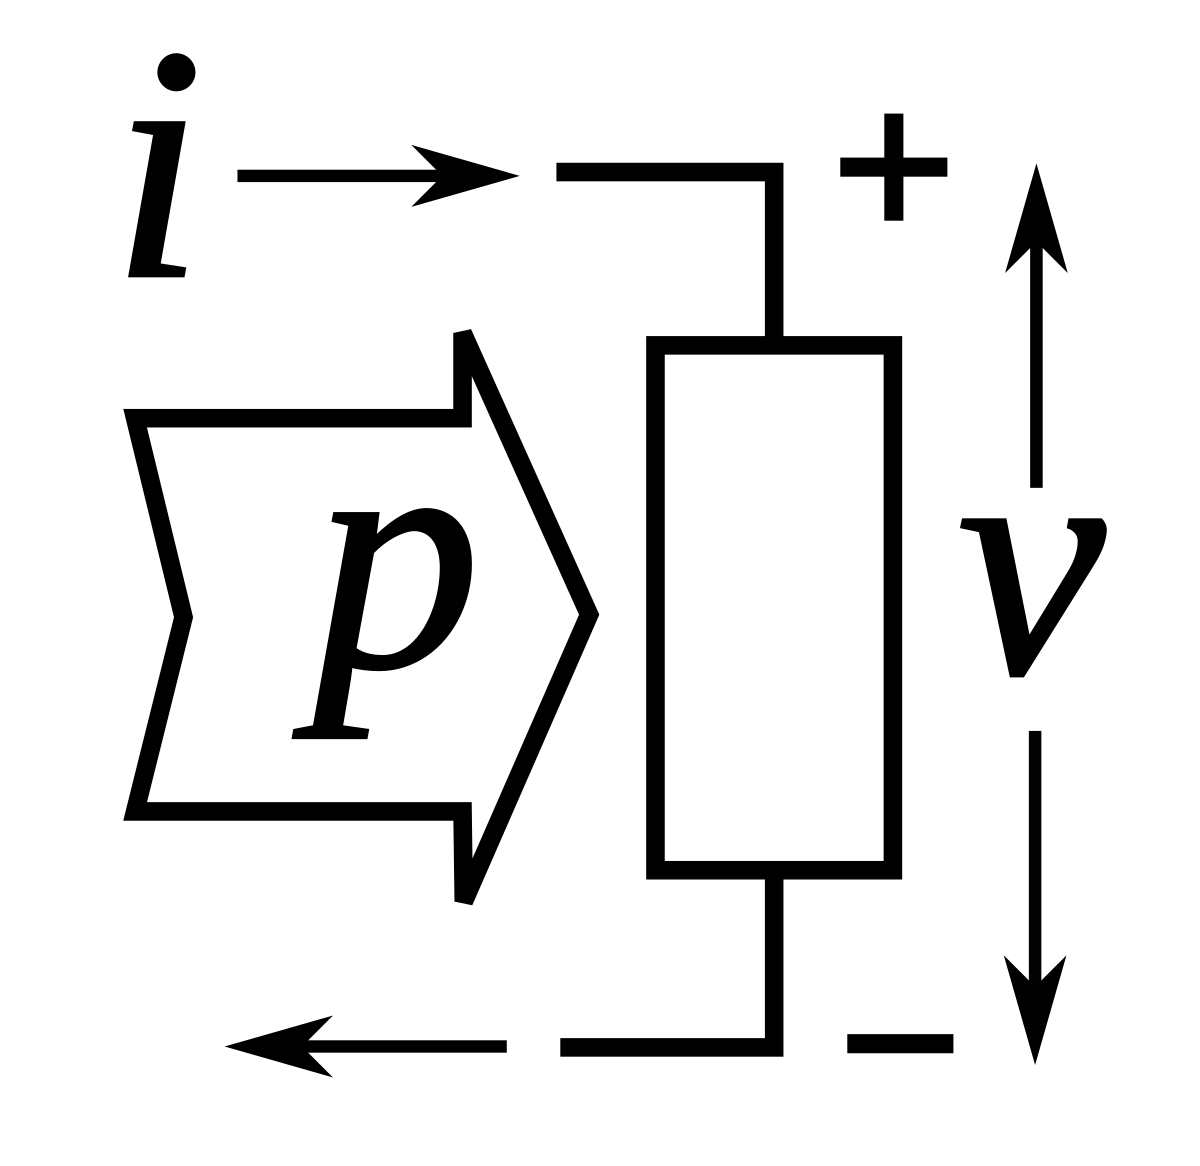
\includegraphics{images/Passive_sign_convention.svg.png}
    \caption{Passive sign convention}
    \label{fig:psc} 
\end{marginfigure}
It's useful to have an idea of the components of circuit
schematics (visual representations of a circuit). Below is a list 
of the terms that will be used in this course:
\begin{itemize}
    \item Elements: The term elements means "components and sources."
    \item Symbols: Elements are represented in schematics by symbols. 
    Symbols for common 2-terminal elements are displayed to the right.
    
\begin{marginfigure}
    \centering
    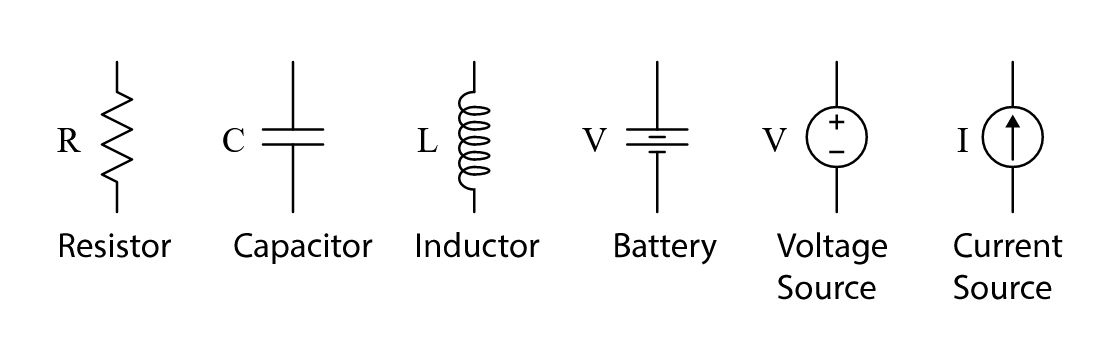
\includegraphics{images/symbols.png}
    \caption{Common circuit symbols}
    \label{fig:symbols}
\end{marginfigure} 

    \item Lines: Connections between elements are drawn as lines, 
    which we often think of as "wires". On a schematic, 
    these lines represent perfect conductors with zero resistance. 
    Every component or source terminal touched by a line is at the same voltage.
    \item Dots: Connections between lines can be indicated by dots. 
    Dots are an unambiguous indication that lines are connected. 
    If the connection is obvious, you don't have to use a dot.
\end{itemize}
Check out the circuit schematic below and see how many components you 
can identify!
\begin{center}
    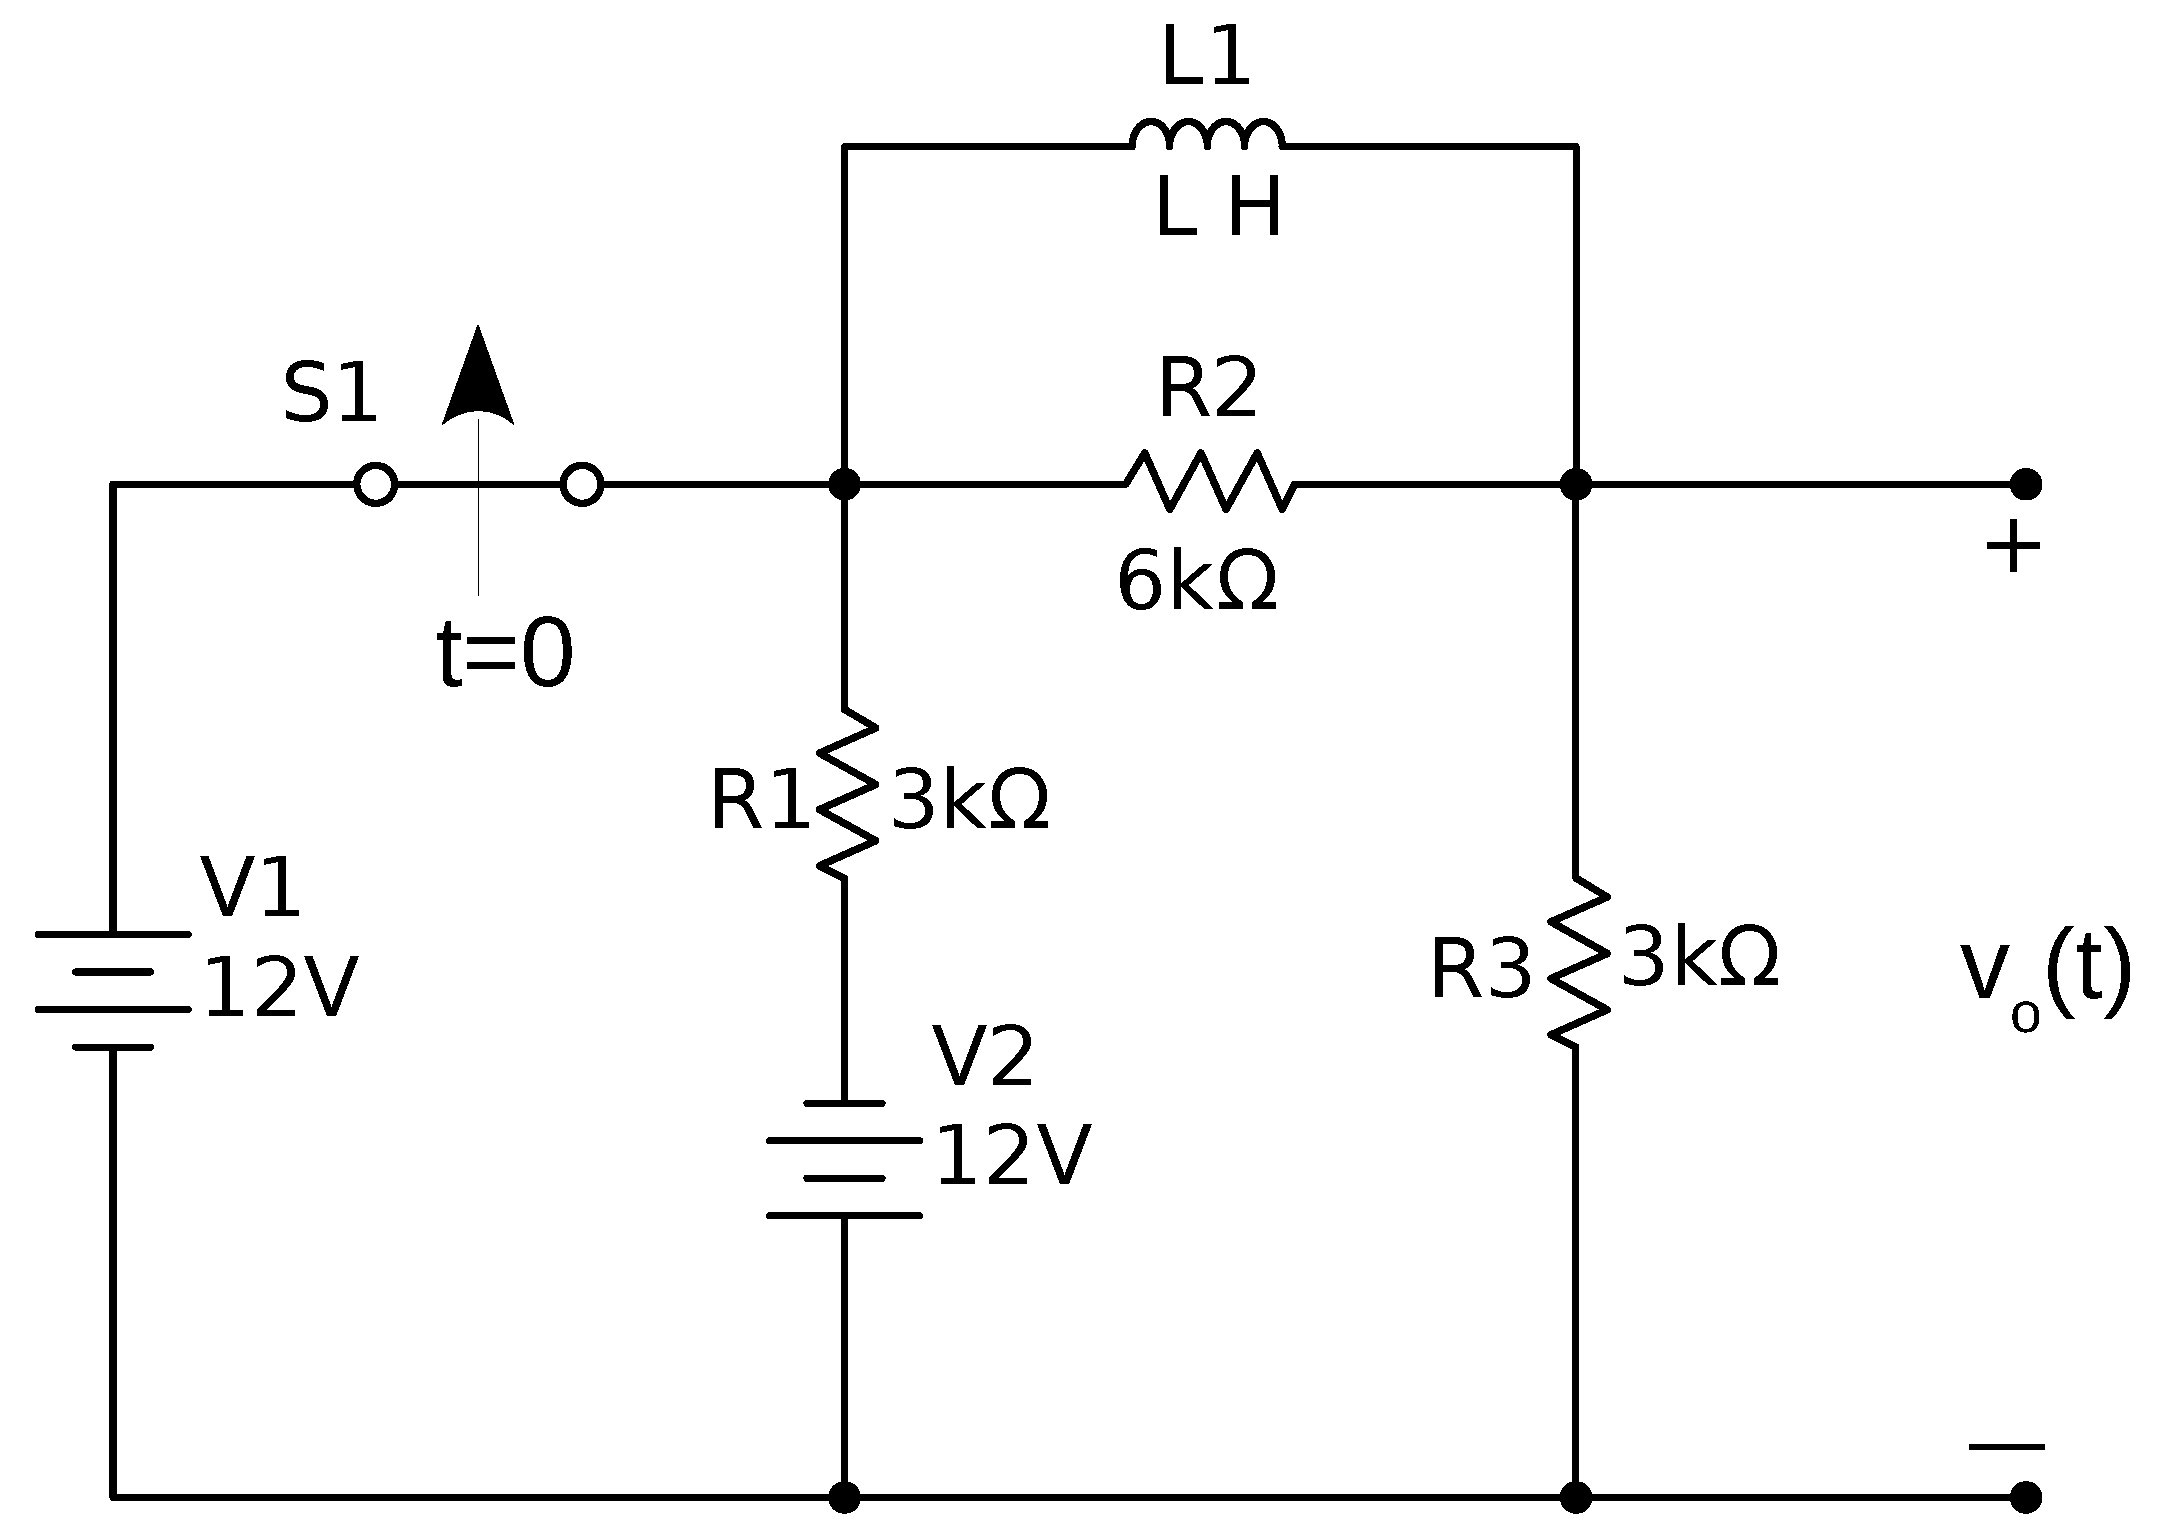
\includegraphics[width=\textwidth/2]{images/PS0_CapacitorCircuit.png}
\end{center}

\pagebreak 

\section{(In)dependent sources, connections, resistance and Ohm's Law}
Now, on to what circuits are doing. For interesting things
to happen we need electrons flowing through those wires,
and for that we need sources. There are two types: independent and dependent.
Independent sources are voltage sources or current sources 
that maintain a constant value regardless of the rest of the 
circuit. They are not influenced by the circuit's current or 
voltage conditions. There are two main types of independent 
sources:
\begin{itemize}
    \item \defn{Independent voltage source}{Maintains a constant 
    voltage across its terminals, regardless of the current 
    flowing through it. It is typically represented by a 
    symbol with a plus sign and a minus sign, indicating 
    the polarity of the voltage.} A battery maintaining a constant
    voltage of 9 V is an example of an independent voltage source.
    \begin{marginfigure}
        \centering
        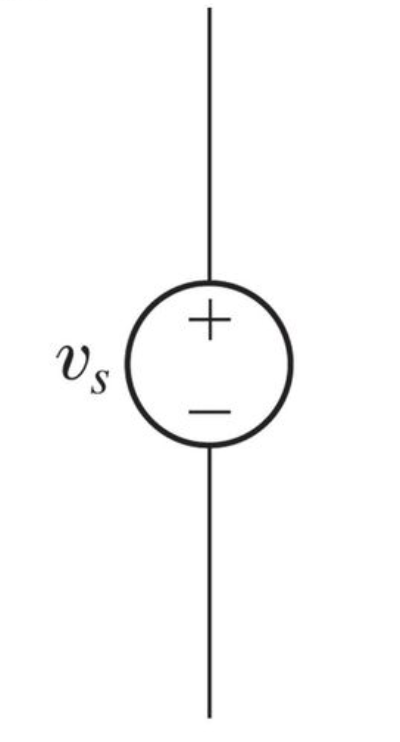
\includegraphics[width=\textwidth/2]{images/independentvoltagesource.png}
        \caption{inependent voltage source}
        \label{fig:independentvoltagesource}
    \end{marginfigure} 

    \item \defn{Independent current source}{Maintains a constant 
    current through its terminals, regardless of the 
    voltage across it. It is usually represented by 
    a symbol with an arrow indicating the 
    direction of current flow.} Consider a current source that 
    provides a constant current of 2 amperes. This source 
    will deliver a current of 2A through any component 
    connected to it, regardless of the 
    voltage across the component.
    \begin{marginfigure}
        \centering
        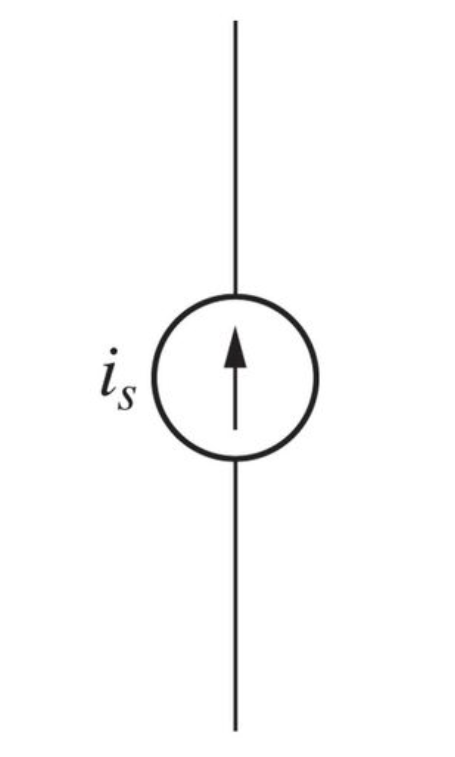
\includegraphics[width=\textwidth/2]{images/independentcurrentsource.png}
        \caption{Independent current source}
        \label{fig:independentcurrentsource}
    \end{marginfigure} 
    
\end{itemize}
Contrasted with independent sources are 
dependent sources. Dependent sources are sources 
whose values are 
dependent on other variables within the circuit. 
These sources are used to model components whose 
behavior changes according to the conditions in 
the circuit. There are four types of dependent sources:
\begin{itemize}
    \item \defn{Voltage-Controlled Voltage Source (VCVS)}{
    This type of dependent source generates a voltage 
    that is proportional to the voltage across a 
    separate part of the circuit.}
    \begin{marginfigure}
        \centering
        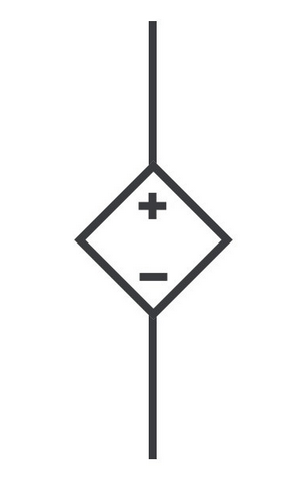
\includegraphics[width=\textwidth/2]{images/dependentvoltagesource.png}
        \caption{Dependent voltage source}
        \label{fig:dependentvoltagesource}
    \end{marginfigure} 

    \item \defn{Current-Controlled Current Source (CCCS)}{
    This type of dependent source generates a current 
    that is proportional to the current flowing 
    through a different part of the circuit.}
    \begin{marginfigure}
        \centering
        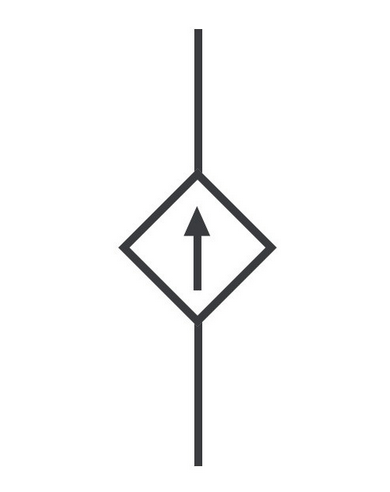
\includegraphics[width=\textwidth/2]{images/dependentcurrentsource.png}
        \caption{Dependent current source}
        \label{fig:dependentcurrentsource}
    \end{marginfigure} 


    \item \defn{Voltage-Controlled Current Source (VCCS)}{
    This type of dependent source generates a 
    current that is proportional to the 
    voltage across a different part of the 
    circuit.}
    \item \defn{Current-Controlled Voltage Source (CCVS)}{
    This type of dependent source generates a 
    voltage that is proportional to the 
    current flowing through a separate part 
    of the circuit.}
\end{itemize}
In both the independent and dependent case, we assume
the sources are ideal. There are two
critical attributes of ideal sources. First, their value remains unchanged indefi-
nitely. Second, they can deliver any amount of power needed by their loads.
Turning off a voltage source is equivalent to replacing it with a 
short circuit (line). Turning off a current source is equivalent to replacing it with an
open circuit (broken line). Also equivalent to an open
circuit is a resistor with infinite resistance. 
Resistance is a measure of how hard it is to shove current
through a resistor. The harder it is, the higher the
resistance. It's given by $R = \frac{\rho L}{A} = \frac{V}{I}$, where $\rho$ 
is the resistivity, $L$ is the length of the resistor, and $A$ is the 
cross-sectional area of the resistor. The reciprocal of
resistance is conductance ($G = \frac{1}{R}$). We can relate 
voltage, current and resistance with \emph{Ohm's Law}.

\defn{Ohm's Law}{$V = IR$.} This law is fundemental to EE and will
occur repeatedly throughout the course. 

\pagebreak 

\section{Kirchhoff's Laws, resistor combinations, and voltage/current division}
\defn{Kirchhoff's Current Law}{The sum of all currents going into
a node is 0. Mathematically, $\sum_k i_k = 0$}. We may intuit 
this by imagining electricity as water flowing into a pipe. Anything that flows 
in must flow out.
Say you have a circuit such as fig. \ref{fig:kcl}. 
\begin{figure}
    \center
    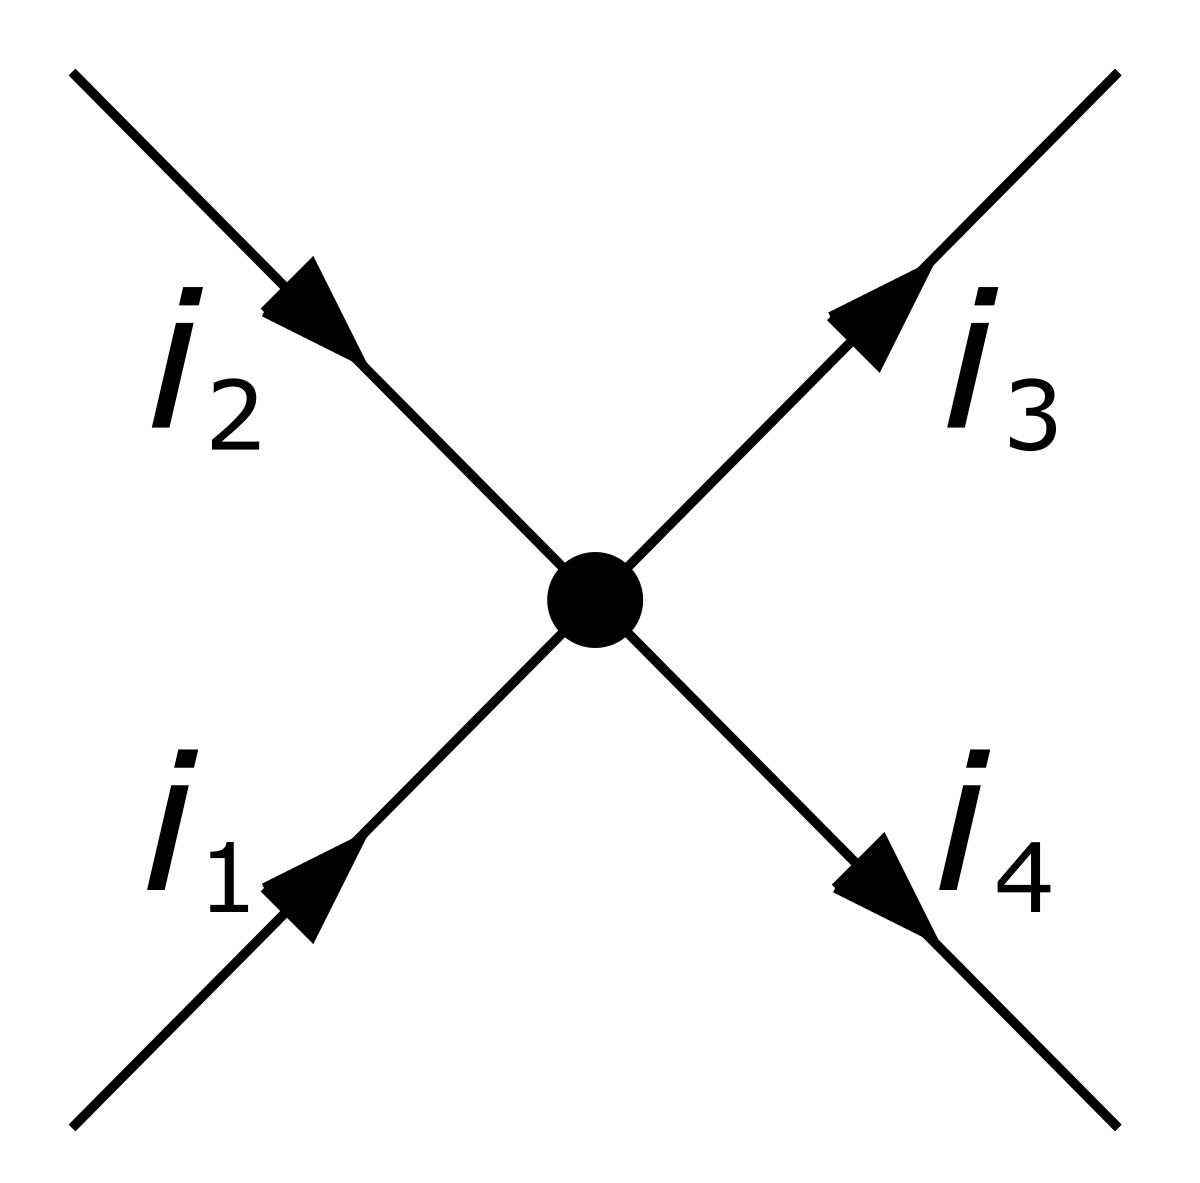
\includegraphics[width=\textwidth/2]{images/1200px-Kirchhoff's_Current_Law.svg.png}
    \caption{Kirchhoff's Current Law}
    \label{fig:kcl}
\end{figure}
By Kirchhoff's
current law, we see that $i_1+i_2-i_3-i_4 = 0 \rightarrow i_1 + i_2 = i_3 +i_4$.
The neat thing is that this must be true for any node in a circuit. 
If you have a node with two known currents going in and one unkown comming out,
Kirchhoff's current law tells us the unknown current is simply the sum
of the known currents. 

Contrasted with Kirchhoff's current law, we have Kirchhoff's voltage
law. 

\defn{Kirchhoff's Voltage Law}{In a closed loop, the sum
of all voltage drops is zero. Mathematically, $\sum_k v_k = 0$}.
A useful way to visualize this is to think of voltage as potential energy.
No matter where you go and how the voltage drops and rises, 
when you get back to where you began, the voltage must be the same
there. You end up with the same gravitational potential if
you return to the same spot, even if you run up and down a mountain.
Imagine a closed loop such as fig. \ref{fig:series}.
Say the voltage across the battery is $15V$ and each resistor
is identical. Although we don't know for sure yet, we can guess
that the current will be the same through each, and ergo
by Ohm's Law ($V=IR$) so will each voltage. Therefore,
\[15 + 3V = 0 \rightarrow V = -5\]

Now that we have a good idea of circuit components and how voltage/current behave, we can look 
at important configurations. These are the most useful:

\defn{Series Combination}{In a series combination, the elements 
are connected with end to end in contact}. We can use Kirchhoff's current
law to show that the current at each point in the circuit is the same. Since current 
flows into a resistor it has no option but to flow out the same resistor.
\begin{figure}
    \center
    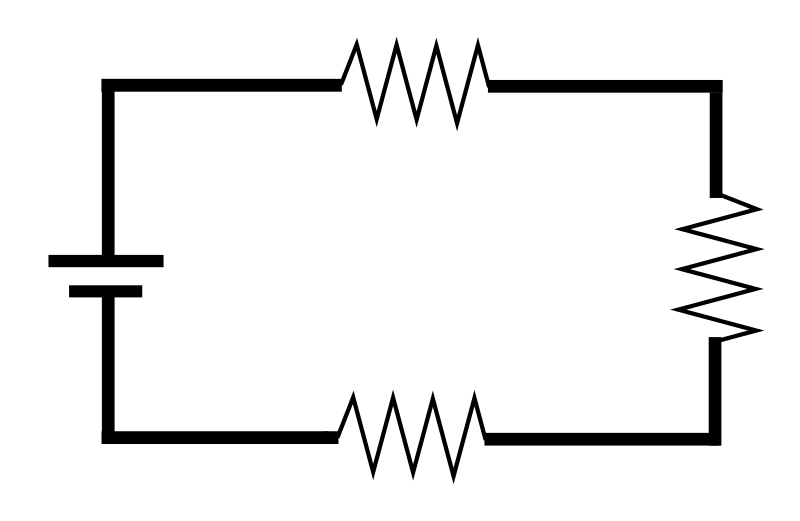
\includegraphics[width=\textwidth/2]{images/Series_circuit.svg.png}
    \caption{Series Combination}
    \label{fig:series}
\end{figure}
Say the resistances are $R_1, R_2$, and $R_3$. By Kirchhoff's voltage law, we have
\begin{align*}
    V &= IR_1 + IR_2 + IR_3\\
    &= I(R_1 + R_2 + R_3) \\
    &= IR_{total} \\
    &\rightarrow R_{total} = R_1 + R_2 + R_3\\
\end{align*}
Therefore for resistors in series, the total resistance is 
equal to the sum of each individual resistance. 

\defn{Parallel Combination}{When two or more resistances are 
connected between the same two points, they are said to be 
connected in parallel. Here, voltage is equal
across all elements}. 
\begin{figure}
    \center
    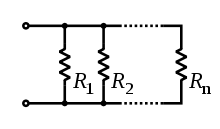
\includegraphics[width=\textwidth/2]{images/220px-Resistors_in_parallel.svg.png}
    \caption{Parallel Combination}
    \label{fig:parallel}
\end{figure}
In fig. \ref{fig:parallel}, the total current is split among
$n$ different resistors. That is, $I = \sum_k^n i_k$. With a bit of
manipulation and Ohm's Law, we have that
\begin{align*}
    I &= \frac{V}{R_{total}}\\
    &= \sum_k^n i_k \\
    &= \sum_k^n V/R_k \\
    &\rightarrow \frac{1}{R_{total}} \\
    &= \sum_k^n \frac{1}{R_k} \\
\end{align*}

So for resistors in parallel, the reciprocal of the total resistance is 
the sum of the reciprocals of the individual resistances. 

Now would
be an excellent point to introduce the idea of 

\pagebreak 

\section{Equivalent resistance}

\defn{Equivalent resistance}{a simplification
of a circuit with multiple resistors, where the resistance
of the equivalent resistor maintains the same voltage 
and current relationship.} We have already seen formulas
for when the resistors are in parallel or series, and can
use them to determine the equivalent resistance across two nodes.
For instance, consider fig. \ref{fig:seriesandparallelequi}.
\begin{figure}

    \caption{Finding equivalent resistance in circuit with 
    resistors in series and parallel, step 1}
    \center
    \label{fig:seriesandparallelequi}
    \begin{circuitikz}
        % Circuit code
        \draw (0,0)node[left=0.2cm]{B} 
            to[short,o-] ++(1,0) coordinate(b1) 
            to[short] ++(3,0) coordinate (b2) 
            to[short] ++ (2.5,0) 
            to[R,l_=$\SI{1.5}{\kilo\ohm}$] ++(0,2.5)  coordinate (c1) 
            to[R,l_=$\SI{3}{\kilo\ohm}$] ++(0,2.5) 
            to[short] ++(-2.5,0) coordinate (a2) 
            to[R,l_=$\SI{1}{\kilo\ohm}$]++(-3,0) coordinate (a1) 
            to[short,-o] ++(-1,0) node[left=0.2cm]{A} ;
         
        \draw (a1) to[R,l_=$\SI{10}{\kilo\ohm}$,*-*] (b1);
         
        %\draw (c1) to[R,l_=$\SI{5}{\kilo\ohm}$,*-] ++ (-2.5,0)coordinate (c2);
         
        \draw (c1) ++ (-2.5,0) to[R,l=$\SI{2}{\kilo\ohm}$,-*] (a2);
        \draw (c1) ++ (-2.5,0) to[R,l_=$\SI{5}{\kilo\ohm}$,*-*] (b2);
         
    \end{circuitikz}
\end{figure}
We can see that the $1 \Omega$ and the $10 \Omega$ resistor are in series, 
so their equivalent resistance is simply $1 + 10 \Omega = 11 \Omega$. We can condense the
circuit to fig \ref{fig:seriesandparallelequi2}. 
\begin{figure}

    \caption{Finding equivalent resistance in circuit with 
    resistors in series and parallel, step 2}
    \center
    \label{fig:seriesandparallelequi2}
    \begin{circuitikz}
        % Circuit code
        \draw (0,0)node[left=0.2cm]{B} 
            to[short,o-] ++(1,0) coordinate(b1) 
            to[short] ++(3,0) coordinate (b2) 
            to[short] ++ (2.5,0) 
            to[R,l_=$\SI{1.5}{\kilo\ohm}$] ++(0,2.5)  coordinate (c1) 
            to[R,l_=$\SI{3}{\kilo\ohm}$] ++(0,2.5) 
            to[short] ++(-2.5,0) coordinate (a2) 
            to[short] ++(-3,0) coordinate (a1)
            to[short,-o] ++(-1,0) node[left=0.2cm]{A} ;
         
        \draw (a1) to[R,l_=$\SI{11}{\kilo\ohm}$,*-*] (b1);
         
        \draw (c1) ++ (-2.5,0) to[R,l=$\SI{2}{\kilo\ohm}$,-*] (a2);
        \draw (c1) ++ (-2.5,0) to[R,l_=$\SI{5}{\kilo\ohm}$,*-*] (b2);
    \end{circuitikz}
\end{figure}
We next combine the $2 \Omega$ and the $5 \Omega$ resistor to obtain an
equivalent resistance of $7 \Omega$, and the $3 \Omega$ and the $1.5 \Omega$
to obtain $4.5 \Omega$ (fig. \ref{fig:seriesandparallelequi3})
\begin{figure}

    \caption{Finding equivalent resistance in circuit with 
    resistors in series and parallel, step 3}
    \center
    \label{fig:seriesandparallelequi3}
    \begin{circuitikz}
        % Circuit code
        \draw (0,0)node[left=0.2cm]{B} 
            to[short,o-] ++(1,0) coordinate(b1) 
            to[short] ++(3,0) coordinate (b2) 
            to[short] ++ (2.5,0) 
            to[R,l_=$\SI{1.5}{\kilo\ohm}$] ++(0,5)  coordinate (c1) 
            to[short] ++(-2.5,0) coordinate (a2) 
            to[short] ++(-3,0) coordinate (a1)
            to[short,-o] ++(-1,0) node[left=0.2cm]{A} ;
         
        \draw (a1) to[R,l_=$\SI{11}{\kilo\ohm}$,*-*] (b1);
         
        \draw (c1) ++ (-2.5,0) to[R,l=$\SI{2}{\kilo\ohm}$,-*] (b2);
    \end{circuitikz}
\end{figure}
Now that we are left with only resistors in parallel, we may use the formula
$\frac{1}{R_{eq}} = \sum_k \frac{1}{R_k}$ to obtain 
$\frac{1}{R_eq} = \frac{1}{11} + \frac{1}{2} + \frac{1}{1.5} = \frac{83}{66}$,
yielding $R_{eq} = \frac{66}{83} \Omega$. 
Note that this method is only possible when the circuit has 
resistors in series or parallel. For more complex situations, such as
when souces are present or resistors are combined in neither
series nor parallel, we must use Kirchhoff's laws and good judgement 
to find the equivalent resistance. Consider fig. \ref{fig:eqresources}, where 
we have a circuit with both dependent and independent sources. 
\begin{figure}
    \caption{Finding equivalent resistance in cirucit with sources}
    \label{fig:eqresources}
    \begin{circuitikz}[american currents, american voltages]
        % Circuit code
        \draw (0,0)node[left=0.2cm]{B}
            to[short,o-] ++(0.5,0) coordinate (b1)
            to[short,] ++(2,0) coordinate (b2)
            ;
        \draw (0,2)node[left=0.2cm]{A}
            to[short,o-] ++(0.5,0) coordinate (a1)
            ;
        \draw to[short] (b1) (a1)
            (b1) to[I, l_=$3A$] (a1)
            ;
        \draw (a1) to[short] ++ (0.5,0)
            to[R,l^=$\SI{4}{\ohm}$, v_>=$V_1$] ++(1,0)   
            to[short] ++ (0.5,0) coordinate (a2)
            ;
        \draw (b2) to [cI, l_=$(0.25 S) V_1$] (a2);
        \draw (a2) to[short] ++(3,0) coordinate (a3)
            (a3) to[R,l^=$\SI{8}{\ohm}$] ++(0,-2) coordinate (b3)
            (b3) to[short] (b2)
            ;
    \end{circuitikz}
\end{figure}
The process for finding the equivalent resistance of a circuit 
with sources is as follows:
\begin{enumerate}
    \item "Turn off" all independent sources. That is, replace independent current sources with
    opens and independent voltage sources with shorts. 
    \item Apply a test current or voltage across $a$ and $b$.
    \item Use $R_{eq} = \frac{V_test}{I_test}$, circuit laws, and algebra to solve. 
\end{enumerate}
Let's apply a test current of $1 A$ across $a,b$, as shown in fig. \ref{fig:eqresources2}
\begin{figure}
    \caption{Finding equivalent resistance in cirucit with sources}
    \label{fig:eqresources2}
    \begin{circuitikz}[american currents, american voltages]
        % Circuit code
        \draw (0,0)node[left=0.2cm]{B}
            to[short,o-] ++(0.5,0) coordinate (b1)
            to[short,] ++(2,0) coordinate (b2)
            ;
        \draw (0,2)node[left=0.2cm]{A}
            to[short,o-] ++(0.5,0) coordinate (a1)
            ;
        \draw (0,0) to[I, l_=$3A$] (0,2);
        \draw (a1) to[short] ++ (0.5,0) 
            to[R,l^=$\SI{4}{\ohm}$, v_>=$V_1$] ++(1,0)   
            to[short] ++ (0.5,0) coordinate (a2)
            ;
        \draw (b2) to [cI, l_=$(0.25 S) V_1$] (a2);
        \draw (a2) to[short] ++(3,0) coordinate (a3)
            (a3) to[R,l^=$\SI{8}{\ohm}$] ++(0,-2) coordinate (b3)
            (b3) to[short] (b2)
            ;
        \draw (a2) node[above]{x};
        \draw (a3) to [short,i>=$I_y$] ++(0,-0.25);
    \end{circuitikz}
\end{figure}
By using Kirchhoff's voltage law
on the outermost loop, we have 
\[V_{test} = V_1 + 8 I_y\]
We also know that the current flowing into node $x$ must be 
equal to the current flowing out. That is, 
\[1 + (0.25 S)V_1 =I_y\]
But since we know $R_1$ and $I_1$, we can find $V_i$. We simply have 
\[V_1 = 1 A \times 4 \Omega = 4 V\]
Meaning 
\[I_y = 4 * 0.25 + 1 = 2\]
We can plug $V_1$ and $I_y$ into $V_{test} = V_1 + 8 I_y$ to get $V_{test} = 4 + 16 = 20$,
and via $R_{eq} = \frac{V_{test}}{I_{test}}$ we have $R_{eq} = \frac{20 V}{1 A} = 20 \Omega$.

\pagebreak 

\section{Analysis}
Let's now examine a couple of extremely powerful techniques we can use 
to analyze circuits, \emph{nodal analysis} and \emph{mesh analysis}.  

\defn{Nodal analysis}{a systematic method used to determine the voltage at every 
(essential) node in a circuit. After picking our reference (ground) node, we
systematically apply KCL at every (essential) node in the circuit except,
of course, for the ground node. By finding every nodal voltage in the circuit, 
we can find every branch current, which enables us to determine the
power absorbed or delivered by every element. Because of its ability to
be applied to any circuit, nodal analysis is the method most often used
in circuit analysis computer programs}. Here are the steps to perform nodal 
analysis: 
\begin{enumerate}
    \item Number all (essential) nodes of the given circuit.
    \item Write KCL for every (essential) node by keeping in mind that only nodal
    voltages should be used (no currents). If other unknowns are involved (e.g.
    dependent source equations) express them as a function of the unknown
    nodal voltages (e.g. by using Ohm's law).
    \item Group the resulting equations together in a matrix form.
    \item Solve for the unknown nodal voltages by inverting the resulting linear
    equation.
    \item Calculate any quantity of interest (e.g power consumption) from the
    known nodal voltages.
\end{enumerate}
Consider an example cirucit, fig. \ref{fig:nodalanal}.
\begin{figure}
    \caption{Using nodal analysis}
    \label{fig:nodalanal}
    \begin{circuitikz}[american currents, american voltages]
        \draw (0,0) to[I, l_=$I_{s_1}$] (0,3) coordinate (a1)
            to[short,-o] ++(2,0) coordinate (a2)
            to[R, l=$R_2$] ++(2,0) coordinate (a3)
            to[short] ++(2,0) coordinate (a4)
            to[V, l=$V_{s_3}$] ++(0,-3) coordinate (b4)
            (b4) to (3,0) node[ground]{}
            (3,0) to[short] (0,0)
            (a2) to[R, l=$R_1$] (2,0)
            (a3) to[I, l=$I_{s_2}$] (4,0)
            ;
        \draw (a2) node[above]{$V_1$};
        \draw (a3) node[above]{$V_2$};
    \end{circuitikz}
\end{figure}
Let's apply our steps to find the nodal voltages $V_1$ and $V_2$.
\begin{enumerate}
    \item Number the essential nodes (fig. \ref{fig:nodalanal2}).
    \begin{figure}
        \caption{Numbering nodes}
        \label{fig:nodalanal2}
        \begin{circuitikz}[american currents, american voltages]
            \draw (0,0) to[I, l_=$I_{s_1}$] (0,3) coordinate (a1)
                to[short,-o] ++(2,0) coordinate (a2)
                to[R, l=$R_2$] ++(2,0) coordinate (a3)
                to[short] ++(2,0) coordinate (a4)
                to[V, l=$V_{s_3}$] ++(0,-3) coordinate (b4)
                (b4) to (3,0) node[ground]{}
                (3,0) to[short] (0,0)
                (a2) to[R, l=$R_1$] (2,0)
                (a3) to[I, l=$I_{s_2}$] (4,0)
                ;
            \draw (a2) node[above]{1};
            \draw (a3) node[above]{2};
        \end{circuitikz}
    \end{figure}
    \item Apply Kirchhoff's current law to each node
    \begin{align*}
        -I_{s_1} - \frac{0-V_1}{R_1} - \frac{V_2-V_1}{R_2} &= 0\\
    \end{align*}
    Here we can actually take a shortcut. Since the negative terminal 
    of $V_{s_3}$ is grounded, then the voltage at the positive terminal 
    must be $V_{s_3}$. Since this terminal is connected directly to $V_2$, 
    we know that $V_2 = V_{s_3}$. That makes our equations
    \begin{align*}
        -I_{s_1} - \frac{0-V_1}{R_1} - \frac{V_2-V_1}{R_2} &= 0\\
        V_2 &= V_{s_3} \\
    \end{align*}
    \item Let's group these by the variables we wish to find now. 
    \begin{align*}
        V_1(\frac{1}{R_1} + \frac{1}{R_2}) - V_2\frac{1}{R_2} &= I_{s_1}\\
        0V_1 + V_2 &= V_{s_3} \\
    \end{align*}
    Which in matrix form becomes
    \[ \begin{bmatrix}
        \frac{1}{R_1} + \frac{1}{R_2} & -\frac{1}{R_2} \\
        0 & 1
    \end{bmatrix}
    \begin{bmatrix}
        V_1 \\
        V_2
    \end{bmatrix}
     =
    \begin{bmatrix}
        I_{s_1} \\
        V_{s_3}
    \end{bmatrix} \]
    \item From here, we could use a computer program to find the inverse matrix
    and multiply both sides by it to get the vector [$V_1$, $V_2$] by itself. 
    I'm not going to do this because I'm lazy, but if you're interested try 
    using Mathematica or MATLAB. 
\end{enumerate}

If our circuit lacks a ground, we may simply choose some node as ground, since
voltages are relative and having a grounded node makes analysis easier. 

%Super nodes?

%Modified nodal analysis

\defn{Mesh analysis}{This method is used to determine every loop current in a circuit. We
use KVL around meshes (loops) to find the mesh (loop) currents. We
can then calculate any voltage or any branch current from the resulting
mesh currents. (Basic) mesh analysis has a limitation in that it can only
be applied to planar circuits}.

Here are the steps to perform mesh analysis: 
\begin{enumerate}
    \item Choose your loops and draw mesh currents in them. 
    \item Use Kirchhoff's voltage law and the voltages you encounter 
    to create a system of equations. If two mesh currents 
    go against each other, the net current is their difference. 
    \item Group the resulting equations together in a matrix form.
    \item Solve for any quantity of interest. 
\end{enumerate}

Note that you don't want two mesh currents flowing through the same 
current source. If you find a circuit where this occurs, make a 
larger loop where no current sources are shared. 

\pagebreak 

\section{Source transformations}
\defn{Source transformation}{Source transformation is a 
wonderful tool that can be used to change the
originally given circuit to an equivalent and simpler circuit}.
Two important theorems are Thevenin's theorem and Norton's theorem.

\defn{Thevenin's theorem}{states that it 
is possible to simplify any linear circuit, irrespective of 
how complex it is, to an equivalent circuit with a single 
voltage source and a series resistance}. 
\begin{figure}
    \caption{Thevenin equivalent}
    \label{fig:thevenin}
    \begin{circuitikz}[american currents, american voltages]
        \draw (0,0) to[V, v=$V_{s}$, invert] (0,3) coordinate (a1)
            to[R, l=$R_s$, -o] ++(2,0) coordinate (a2);
        \draw (0,0) to[short, -o] (2,0);
    \end{circuitikz}
\end{figure}
Here are the steps to find the Thevenin equivalent circuit:
\begin{enumerate}
    \item Remove the load resistor.
    \item Find $R_{th}$ by shorting all voltage sources and 
    by open circuiting all the current sources and then see what 
    the resistance looks like from the point of view of the nodes 
    where the load resistor was located.
    \item Find $V_{Th}$ by finding the voltage across the nodes the load was 
    originally hooked to, using standard circuit analysis methods.
    \item Replace the load and find the current 
    flowing through the load with these new values.
\end{enumerate}
\defn{Norton's theorem}{states that any 
linear circuit can be simplified to an equivalent circuit 
consisting of a single current source and parallel resistance 
that is connected to a load}.
\begin{figure}
    \caption{Norton equivalent}
    \label{fig:norton}
    \begin{circuitikz}[american currents, american voltages]
        \begin{circuitikz}[american currents, american voltages]
            \draw (0,0) to[I, l_=$I$] (0,3) coordinate (a1)
                to[short] ++(2,0) coordinate (a2);
            \draw (0,0) to[short] (2,0)
                to[R, l=$R_s$] ++(0,3);
            \draw (2,3) to[short, -o] (3,3);
            \draw (0,0) to[short, -o] (3,0);
        \end{circuitikz}
    \end{circuitikz}
\end{figure}
Here are the steps to find the Norton equivalent circuit: 
\begin{enumerate}
    \item Remove the load resistor and replace it with a short circuit.
    \item Find $I$ by calculating the current through the short circuit where the load was.
    \item Find $R$ by creating an open circuit where the load resistor is, 
    shorting all voltage sources and by open circuiting all the current sources. 
    Once this is done, calculate the resistance seen by the open circuit.
    \item Replace load and find the current flowing through the load or 
    voltage across the load with these new values.
\end{enumerate}
Essentially, there are three quantities
we may be interested in finding. 
\begin{itemize}
    \item[($R_{eq}$)] Turn off all independent sources (dependent
    sources remain unchanged) and calculate the resulting resistance at the
    desired port. Notice that you may have to apply the i-v test if resistors
    cannot be combined through series and parallel connections, or if the
    circuit includes dependent sources.
    \item[($V_{th}$)] Leave the desired port open-circuited
    (i.e. no load connected) and find the voltage across it.
    \item[($I_N$)] Short-circuit the desired port (i.e. connect
    a short circuit across the port) and find the current through it. 
\end{itemize}
Let's see how to transform between Norton and Thevenin circuits. Fig. \ref{fig:tnsimp}
shows a circuit with one voltage source and a resistor in series. 
\begin{figure}
    \caption{Thevenin to Norton}
    \label{fig:tnsimp}
    \begin{circuitikz}[american currents, american voltages]
        \draw (0,0) to[V, v=$V_{s}$, invert] (0,3) coordinate (a1)
            to[R, l=$R_s$, -o] ++(2,0) coordinate (a2);
        \draw (0,0) to[short, -o] (2,0);
    \end{circuitikz}
\end{figure}
This series resistance normally represents the internal 
resistance of a practical voltage source.
Let us short circuit the output terminals of the 
voltage source circuit as shown in fig. \ref{fig:tnsimp2}
\begin{figure}
    \caption{Thevenin to Norton}
    \label{fig:tnsimp2}
    \begin{circuitikz}[american currents, american voltages]
        \begin{circuitikz}[american currents, american voltages]
            \draw (0,0) to[V, v=$V_{s}$, invert] (0,3) coordinate (a1)
                to[R, l=$R_s$, -o] ++(2,0) coordinate (a2);
            \draw (0,0) to[short, -o] (2,0)
                to[short] ++(0,3);
                ;
        \end{circuitikz}
    \end{circuitikz}
\end{figure}
We know that $V_s = I R_s$, where $I$ is the current delivered
by the voltage source when it is short circuited.
Now, let's take a current source of the same current $I$ 
which produces same open-circuit voltage at its open terminals 
as shown in fig. \ref{fig:tnsimp3}
\begin{figure}
    \caption{Thevenin to Norton}
    \label{fig:tnsimp3}
    \begin{circuitikz}[american currents, american voltages]
        \begin{circuitikz}[american currents, american voltages]
            \draw (0,0) to[I, l_=$I$] (0,3) coordinate (a1)
                to[short] ++(2,0) coordinate (a2);
            \draw (0,0) to[short] (2,0)
                to[R, l=$R_t$] ++(0,3);
            \draw (2,3) to[short, -o] (3,3);
            \draw (0,0) to[short, -o] (3,0);
        \end{circuitikz}
    \end{circuitikz}
\end{figure}
Now we have $I = \frac{V_s}{R_t}$, meaning $R_s = R_t$. The open circuit 
voltage of both the sources is $V_s$ and short 
circuit current of both sources is $I$. The 
same resistance connected in series in voltage 
source is connected in parallel in its equivalent current source.
So, the voltage source and current source are equivalent to each other.
Changing between forms is called a source transformation and can be used 
to simplify an electric circuit, since any place a voltage source 
and resistor are in series we can transform to a current source and resistor
in parallel (and vice versa). If the voltage of the voltage source is 
$V_{th}$ and the resistance is $R$, then the current of the equivalent
current source will be $\frac{V_{th}}{R}$.

Let's do an example. 
Say we have the circuit in fig. \ref{fig:tnexample} and we wish to find 
the Thevenin voltage and Norton current with respect to terminals $a$ and $b$.  
\begin{figure}
    \begin{center}
        \begin{circuitikz}[american currents, american voltages]
            \draw (0,0) to[V, v=$30$ V, invert] (0,3) coordinate (a1)
                to[R, i=$I_0$, l=$10\Omega$] ++(3,0) coordinate (a2);
            \draw (0,0) to[short] (3,0) coordinate (b2)
                to[cV, l=$2V_x$, invert] ++(0,3);
            \draw (b2) to ++(1,0) coordinate (b3) node[ground]{}
                (b3) to[short] ++(1,0) coordinate (b4);
            \draw (b4) to[cI, l_=$0.2I_0$] ++(0,3) coordinate (a3)
                (a3) to[short, -o] ++(3,0) coordinate (a4)
                (b4) to[short, -o] ++(3,0) coordinate (b5);
            \draw (a4) to[R, l=$50 \Omega$, v=$V_x$] (b5);
            \draw (a4) node[above]{$a$};
            \draw (b5) node[below]{$b$};
        \end{circuitikz}
    \end{center}
    \caption{Source transformation example}
    \label{fig:tnexample}
\end{figure}
Let's simplify this circuit a bit. First, notice 
that we have $30 - 2V_x$ V across the $10 \Omega$ resistor. 
By Ohm's law, $I_0 = \frac{30 - 2V_x}{10}$. Looking at the right loop,
we have that the current flowing across the resistor is $0.2\frac{30 - 2V_x}{10}$. 
That means $V_x = 50 * 0.2\frac{30 - 2V_x}{10} = 10 \frac{30 - 2V_x}{10}$. Let's
organize our equations. 
\begin{align*}
    I_0 &= \frac{30 - 2V_x}{10} \\
    V_x &= 10 \frac{30 - 2V_x}{10}
\end{align*}
In this case, we don't even need linear algebra to solve. The second equation
yields $V_x = 10$ V. The Norton current is the 
current through $a$ and $b$ when their load resistance is shorted, so let's replace 
that $50 \Omega$ resistor with a short. That makes $V_x = 0$, and using KVL on the 
leftmost loop we find that $-30+2\times0+10I_0=0 \rightarrow I_0 = 3$. The Norton current 
is the current through that short between terminals $a$ and $b$, which is simply 
$0.2 \times 3 = 0.6$ A. Notice that $V_x = V_{th}$ and we are done.  

Well and good, but what if we want to try source transformations? Let's do just that
on circuit \ref{fig:stexample}. 
\begin{figure}
    \center
    \begin{circuitikz}[american currents, american voltages]
        \draw (0,0) to[V, l=$40$ V, invert] (0,3) coordinate (b0)
        to[R, l=$10\Omega$, v=$V_x$] (3,3) coordinate (b1)
        to[short] ++(0,1) coordinate (c1)
        to[I, l=$3$ A] ++(3,0) coordinate (c2)
        to[short] ++(0,-1) coordinate (b2)
        to[short] ++(3,0) coordinate (b3)
        to[cI, l=$2V_x$, invert] ++(0,-3) coordinate (a3);
    \draw (a3) to ++(-4.5,0) node[ground]{}
        to[short] ++(-4.5,0);
    \draw (b1) to[R, l_=$12\Omega$] (b2);
    \draw (b2) to[R, l=$8\Omega$] ++(0,-3);
    \end{circuitikz}
    \caption{Source transformation example}
    \label{fig:stexample}
\end{figure}
We could pretty easily solve this with nodal analysis, but we know that a current source $I$ and resistor $R$ in parallel 
can be simplified to a resistor and an $RI$ voltage source in series. Performing this transformation, 
we have fig. \ref{fig:stexample2}. 
\begin{figure}
    \center
    \begin{circuitikz}[american currents, american voltages]
        \draw (0,0) to[V, l=$40$ V, invert] (0,3) coordinate (b0)
        to[R, l=$10\Omega$, v=$V_x$] (3,3) coordinate (b1)

        to[V, l=$36$ V, invert] ++(1.5,0) coordinate (b2)
        to[R, l_=$12\Omega$] ++(1.5,0) coordinate (b3)

        to[short] ++(3,0) coordinate (b4)
        to[R, l=$8\Omega$] ++(0,-1.5)
        to[cV, l=$16V_x$] ++(0,-1.5) coordinate (a3);
    \draw (a3) to ++(-4.5,0) node[ground]{}
        to[short] ++(-4.5,0);
    \end{circuitikz}
    \caption{Source transformation example, with transformed sources}
    \label{fig:stexample2}
\end{figure}
Now what? Looking at the $10\Omega$ resistor, we see that the 
voltage across it is $40 - 36 = 4$ V. Since this is what we wished to find, we are done. 

\pagebreak 

\section{Linearity, superposition, and max power transfer}
\defn{Linear system}{a linear circuit is one in which the electronic 
components' values (such as resistance, capacitance, inductance, gain, 
etc.) do not change with the level of voltage or current in the circuit}. Linear 
circuits are so called because they can be expressed as a linear combination of
sources. 

\defn{Superposition}{for any linear and bilateral network or circuit with 
multiple independent sources, the response of an element will be equal to the 
sum of the responses of that element by considering one source at a time}. For 
instance, say we have a circuit such as fig. \ref{fig:super}
\begin{figure}
    \center
    \begin{circuitikz}
        \draw (0,0) to[short, i=$I_1$] (3,0)
            to[R, l=$R$] (3,3);
        \draw (0,3) to[short, i=$I_2$] (3,3);
    \end{circuitikz}
    \caption{Superposition}
    \label{fig:super}
\end{figure}
If we want to calculate the voltage across $R$, then we can simply sum the 
currents to get $V = (I_1+I_2)R$ by the principle of superposition. 

Say we have a linear system with two terminals, like fig. \ref{fig:linear}. 
\begin{figure}
    \center
    \begin{circuitikz}
        \draw (0,0) to[short] (0,3)
        to[short] (3,3)
        to[short] (3,0)
        to[short] (0,0);
    \draw (3,1) to[short, -o] (4,1);
    \draw (3,2) to[short, -o] (4,2);
    \end{circuitikz}
    \caption{Linear system with two terminals}
    \label{fig:linear}
\end{figure}
We may be interested in finding the value of $R_L$ that maximizes the power extracted across
the terminals by a load resistor placed there. To see how to do this, let's consider the example fig. \ref{fig:maxpow}. 
\begin{figure}
    \center
    \begin{circuitikz}[american currents, american voltages]
        \draw (0,0) to[R, l=$R$] (0,3)
        to[short] (3,3)
        to[short] (3,0)
        to[V, l=$V$] (0,0);
    \draw (3,1) to[short, -o] (4,1);
    \draw (3,2) to[short, -o] (4,2);
    \draw (4,1) to[R, l_=$R_L$] (4,2);
    \end{circuitikz}
    \caption{Max power extracted}
    \label{fig:maxpow}
\end{figure}
We know that the amount of power dissapated is $P_L = I^2 R_L$. 
Substitute $I=\frac{VTh}{RTh+RL}$ in the above equation, and obtain 
\[P_L = \left( \frac{V_{Th}}{(R_{Th} + R_L)} \right) ^2 R_L.\]
For maximum or minimum, the first derivative will be zero. So, differentiate 
$P_L$ with respect to $R_L$ and make it equal to zero.
\begin{align*}
    \frac{dP_L}{dR_L} &= {V_{Th}}^2 \lbrace \frac{(R_{Th} + R_L)^2 \times 1 - R_L \times 2(R_{Th} + R_L)}{(R_{Th} + R_L)^4} \rbrace = 0 \\
    &\rightarrow (R_{Th} + R_L)^2 -2R_L(R_{Th} + R_L) = 0\\
    &\rightarrow (R_{Th} + R_L)(R_{Th} + R_L - 2R_L) = 0\\
    &\rightarrow (R_{Th} - R_L) = 0 \\
    &\rightarrow R_{Th} = R_L
\end{align*}
Note that this implies $P_{max} = \frac{V_{th}^2}{4R_{th}}$. 

\pagebreak 

\section{Capacitors and inductors}

Summary: 
\begin{enumerate}
    \item The \emph{voltage} of a capacitor is always continous. 
    \item The \emph{current} of an inductor is always continous. 
    \item $I_{cap} = C \frac{dV}{dt}$
    \item $V_{ind} = L \frac{dI}{dt}$
    \item Series capacitance: $\frac{1}{C_{total}} = \frac{1}{C_1} + \frac{1}{C_2} + \dots$
    \item Parallel capacitance: $C_{total} = C_1 + C_2 + \dots$
    \item Series inductor: $L_{total} = L_1+L_2+\dots$
    \item Parallel inductor: $\frac{1}{L_{total}} = \frac{1}{L_1} + \frac{1}{L_1} + \dots$
\end{enumerate}

\defn{Capacitor}{two conducting plates with a gap in between, connected to a voltage source}. 
One plate will have positive charge $Q$ and the other plate will have charge $-Q$. 
The units of capacitance are Faradays.
\begin{figure}
    \center
    \caption{Capacitor}
    \label{fig:cap}
    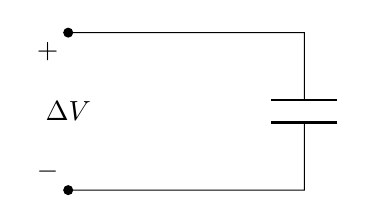
\begin{tikzpicture}
        \draw (0,2) to [short,*-] (3,2) to[C] (3,0) to [short,-*] (0,0);
        \node[below left] at (0,2) {$+$};
        \node[above left] at (0,0) {$-$};
        \node at (0,1) {$\Delta V$};
      \end{tikzpicture}
\end{figure}
The formula for capacitance is $i = C\frac{dV}{dt}$. This formula is true \emph{only if} $V$
is continuous. 

Take the example of a current source hooked up to a capacitor, as in fig. \ref{fig:capcur}. 
\begin{figure}
    \center
    \caption{Capacitor with current source}
    \label{fig:capcur}
    \begin{circuitikz}[american currents, american voltages]
        \draw (0,2) to [short] (3,2) to[C] (3,0) to [short] (0,0);
        \draw (0,0) to[I, l=$I$] (0,2);
      \end{circuitikz}
\end{figure}
Say $C = 0.5 F$. We know that $i = C\frac{dV}{dt}$, so 
\[V(t) = \int_{0}^{t}\frac{I}{C}dt.\] 
If $I = 2t-2$, for example, then we have that 
\begin{align*}
    V(t) &= 4\int_{0}^{t}(2t-2)dt \\
    &= 4t^2-8t
\end{align*}
and we are done. 

Say we have two capacitors in series. It can be shown that 
$\frac{1}{C_{total}} = \frac{1}{C_1} + \frac{1}{C_2}$. Similarly, if 
the capacitors are in parallel instead, $C_{total} = C_1 + C_2$. 

If the reader is familiar with the practical application of capacitors, 
they will know that capacitors are often used to store energy. To see how 
much energy can be stored, recall that $P = IV$ and $I = C\frac{dV}{dt}$. 
Therefore, 
\begin{align*}
    E(t_2)-E(t_1) &= \int_{t_1}^{t_2} P(t) dt \\
    &= \int_{t_1}^{t_2} VC\frac{dV}{dt} \\
    &= \frac{CV^2(t_2)}{2} - \frac{CV^2(t_1)}{2}
\end{align*}

\defn{Inductor}{a passive two-terminal electrical 
component that stores energy in a magnetic field when 
electric current flows through it, according to the 
formula $V = L\frac{dI}{dt}$}. The units of inductance are Henrys (H).
Note that, comparable to capacitors, the given formula is true 
only if \emph{current} is continous. We could show that if the 
current is continuous, then energy stored is equal to $\frac{1}{2}LI^2(t_2) - \frac{1}{2}LI^2(t_1)$
We could also show that for series inductance $L_{total} = L_1+L_2+\dots$
and for parallel inductance $\frac{1}{L_{total}} = \frac{1}{L_1} + \frac{1}{L_1}$. 
To find the equivalent inductance between two terminals, simply turn off all 
independent sources and apply these rules. 

\pagebreak 

\section{First order circuit analysis}

\defn{First order circuit}{contains only one energy storage element 
(capacitor or inductor), and that can, therefore, be described using 
only a first order differential equation}

As we have seen, the three major circuit components are resistors, 
capacitors, and inductors. We can combine these components into 
RC (resistor and capacitor) circuits, LR (inductor and resistor), 
and so on (though if we have more than one energy-storing component then 
we will need a high-order differential equation in order to solve the 
circuit). Recall 
\begin{align*}
    V = L \frac{di}{dt} \\
    i = C\frac{dV}{dt}
\end{align*}
In the steady state, an inductor acts as a short circuit, 
while a capacitor acts as an open circuit. In the first case we 
require that $i$ be continuous and in the second that $V$ be 
continuous. With this information in mind, we can start on first-order 
circuit analysis. Let's see an example with fig. \ref{fig:capvolt}. 
\begin{figure}
    \center
    \caption{Capacitor with voltage source}
    \label{fig:capvolt}
    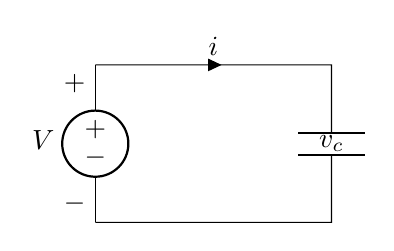
\begin{tikzpicture}[american currents, american voltages]
        \draw (0,2) to [short, i=$i$] (3,2) to[C] (3,0) to [short] (0,0);
        \draw (0,0) to[V, l=$V$, invert] (0,2);
        \node[below left] at (0,2) {$+$};
        \node[above left] at (0,0) {$-$};
        \node at (3,1) {$v_c$};
    \end{tikzpicture}
\end{figure}

It can be shown (I apologize for not showing it) that this circuit
can be modeled by
\begin{align*}
    v_c(t) &= v_c(\infty) +\left(v_c(t_0) - v_c(\infty)\right)e^{(\frac{-1}{RC})(t - t_0)} \\
    &= x(t_0)e^{\lambda (t-t_0)}
\end{align*}
Where $\lambda = \frac{-1}{RC}$ for RC and $-\frac{R}{L}$ for RL (we also have that 
$\lambda = -\frac{1}{\tau}$, where $\tau$ is called the time constant), 
$R_{th}$ is the Thevenin resistance, and $v_c(t)$ is the 
voltage across the capacitor. RC and RL circuits are the only first-order circuits. LC, RLC, and so on all require higher-order
differential equations to solve. 
\marginnote{A useful function to know for diff. eq.s is the \emph{unit step function}, $u(t)$. 
\begin{equation*}
    u(t)=\begin{cases}
              0 \quad &\text{if} \, t < 0 \\
              1 \quad &\text{if} \, t \geq 0 \\
         \end{cases}
\end{equation*}
To change when the function turns off, you can add an offset of $c$, 
like $u(t - c)$. }
In general, the equation for a circuit with a source is 
\[\frac{dx}{dx} = \lambda x + f(t)\]
with solution 
\[x(t_0)e^{\lambda(t - t_0)} + \int_{t_0}^{t} e^{\lambda(t - t_0)} f(\tau) d\tau\]
If the source is constant, the equation becomes 
\[\frac{F}{-\lambda} + (x_0 - \frac{F}{-\lambda}) e^{\lambda(t - t_0)}\]
where $F = f(\tau)$ is constant. This is where the equation 
\[v_c(t) = v_c(\infty) +\left(v_c(t_0) - v_c(\infty)\right)e^{(\frac{-1}{RC})(t - t_0)}\]
comes from. 

Let's see an example. In fig. \ref{fig:foce} the switch has been open for a long time. 
\begin{figure}
    \center
    \caption{First order circuit example}
    \label{fig:foce}
    \begin{circuitikz}[american currents, american voltages]
        \draw (0,0) to[V, l=$10 V$, invert] (0,3)
        to[R, l=$1 \Omega$] (2,3)
        to[short] (3,3)
        (3,3) to[C, l = $1 F$] (3,0)
        ;
        \draw (2,3) to[nos] (2,1.5)
        (2,1.5) to[R, l=$1 \Omega$] (2,0)
        ;
        \draw (3,0) to[short] (0,0);
      \end{circuitikz}
\end{figure}
Thus, at $t_0$, the voltage $v_c(t_0)$ will be equal to the source voltage, 
10. After the switch is closed and sufficient time has passed, the voltage will be across 
the two 1 $\Omega$ resistances, 
which are in series. Therefore $v_c(\infty) = 10 V \times \frac{1 \Omega}{1 \Omega + 1 \Omega} = 5 V$.
Plugging these values into our equation for $v_c(t)$, we get 
\[v_c(t) = 5 +\left(10 - 5\right)e^{(\frac{-1}{RC})(t - t_0)}\]
and all that remains is to find the resistance $R$. $R$ is always calculated with respect to 
the capacitor, so in this case the capacitor will see two resistors in parallel and the total 
resistance will be $(\frac{1}{\frac{1}{1}+\frac{1}{1}}) = 1/2$, so our final equation is 
\[v_c(t) = 5 + 5e^{-2t}\]

\pagebreak 

\section{Response classification}

We may write the general equation for voltage across a capacitor or current across an inductor as 
\[x(\infty) + (x(t_0)-x(\infty))e^{\lambda (t-t_0)}.\]
This can itself be rewritten, as 
\[x(t_0)e^{\lambda (t-t_0)} + x(\infty)(1 - e^{\lambda (t-t_0)})\]
The first term is called the \emph{zero input response}, while the second is 
called the \emph{zero state response}. 

\defn{Zero input response}{the natural 
response of a system to its initial conditions, that is, how the 
system behaves without any external inputs. It is the response 
that arises from the internal dynamics of the system, such as 
the energy stored in its capacitors or inductors}.

\defn{Zero state response}{the output of a system when the input to the system is zero}.

This splitting can be immensely useful when your circuit has sources 
that turn on at different times. The total response will simply be the 
zero input response plus each zero state response. Allow me to show you 
what I mean with the circuit in fig. \ref{fig:response}.
\begin{figure}
    \center
    \caption{Response splitting example}
    \label{fig:response}

    \begin{circuitikz}[american currents, american voltages]
        \draw (0,0) to[V, l=$10u(t)$, invert] (0,3)
        (0,3) to[R, l=$10\Omega$] (2,3)
        (2,3) to[short] (6,3)
        (6,3) to[I, l=$2u(t-100)$, invert] (6,0)
        (6,0) to[short] (0,0)
        ;
        \draw (2,3) to[L, l=$2H$] (2,0)
        ;
        \draw (4,3) to[R, l=$\frac{20}{3}\Omega$] (4,0)
        ;
    \end{circuitikz}
\end{figure}
Say the initial current through the inductor is 
1 amp upwards. Let's build our entire equation 
by finding the zero input response and 
then each of the zero state responses. 
\begin{enumerate}
    \item[Zero input:] Fig. \ref{fig:zir} displays 
    the zero input circuit. 
    \begin{figure}
        \center
        \caption{Zero input response}
        \label{fig:zir}
    
        \begin{circuitikz}[american currents, american voltages]
            \draw (0,0) to[short] (0,3)
            (0,3) to[R, l=$10\Omega$] (2,3)
            (2,3) to[short] (4,3)
            (4,0) to[short] (0,0)
            ;
            \draw (2,3) to[L, l=$2H$] (2,0)
            ;
            \draw (4,3) to[R, l=$\frac{20}{3}\Omega$] (4,0)
            ;
        \end{circuitikz}

    \end{figure}
    From the perspective of the 
    inductor, there is a $10 \Omega$ and $\frac{20}{3} \Omega$
    resistor in parallel, so the total resistance will be $4 \Omega$.
    Thus we have 
    \begin{align*}
        x(t_0)e^{\lambda (t-t_0)} &= I_L(t_0)e^{\frac{-R}{L} (t-t_0)}\\
        &= 1\times e^{\frac{-4}{2} (t-0)} \\
        &= e^{-2t}
    \end{align*}
    as the zero input response. 

    \item[Zero state response for voltage source:] Fig. 
    \ref{fig:vs} displays the circuit for the zero state response 
    in the case of the voltage source. 
    \item[] \begin{figure}
        \center
        \caption{Zero state response for voltage source}
        \label{fig:vs}
    
        \begin{circuitikz}[american currents, american voltages]
            \draw (0,0) to[V, l=$10u(t)$, invert] (0,3)
            (0,3) to[R, l=$10\Omega$] (2,3)
            (2,3) to[short] (4,3)
            (4,0) to[short] (0,0)
            ;
            \draw (2,3) to[L, l=$2H$] (2,0)
            ;
            \draw (4,3) to[R, l=$\frac{20}{3}\Omega$] (4,0)
            ;
        \end{circuitikz}

    \end{figure}
    Let us now calculate the zero state response. At infinity, the inductor will 
    behave as a short circuit and so $I_L(\infty) = \frac{10 V}{10 \Omega} = 1 A$. 
    From the perspective of the inductor, the resistance is again $4 \Omega$. 
    \marginnote{In fact, the resistance in every response will be the same, 
    since the find resistance we turn off every source anyway.}
    \begin{align*}
        x(\infty)(1 - e^{\lambda (t-t_0)}) &= I_L(\infty)(1-e^{\frac{-R}{L}(t-t_0)})\\
        &= 1 \times (1-e^{\frac{-R}{2}(t-0)}) \\
        &= 1-e^{-2t}
    \end{align*}
    But we're not quite done! Because this source turns on at $t=0$, we must multiply the 
    zero state response by $u(t)$, to obtain 
    \[(1-e^{-2t})u(t)\]

    \item[Zero state response for current source:] Fig. 
    \ref{fig:cs} displays the circuit for the current source. 
    \begin{figure}
        \center
        \caption{Zero state response for current source}
        \label{fig:cs}
    
        \begin{circuitikz}[american currents, american voltages]
            \draw (0,0) to[short] (0,3)
            (0,3) to[R, l=$10\Omega$] (2,3)
            (2,3) to[short] (6,3)
            (6,3) to[I, l=$2u(t-100)$, invert] (6,0)
            (6,0) to[short] (0,0)
            ;
            \draw (2,3) to[L, l=$2H$] (2,0)
            ;
            \draw (4,3) to[R, l=$\frac{20}{3}\Omega$] (4,0)
            ;
        \end{circuitikz}

    \end{figure}
    By now we're experts. $R=4$, $L=2$, and $t_0 = 100$, so we already have 
    \begin{align*}
        x(\infty)(1 - e^{\lambda (t-t_0)}) &= I_L(\infty)(1-e^{\frac{-R}{L}(t-t_0)})\\
        &= I_L(\infty) \times (1-e^{\frac{-4}{2}(t-100)})
    \end{align*}
    $I(\infty)$ will simply be the current from the source, $2A$. Ergo, 
    \begin{align*}
        I_L(\infty)(1-e^{\frac{-R}{L}(t-t_0)}) &= I_L(\infty) \times (1-e^{\frac{-4}{2}(t-100)})\\
        &= 2\times (1-e^{-2(t-100)})
    \end{align*}
    Again we must multiply by $u(t-100)$, yielding a final answer of 
    \[2\times (1-e^{-2(t-100)})u(t-100)\]
\end{enumerate}
Putting this all together, we obtain 
\[I_L(t) = e^{-2t} + (1-e^{-2t})u(t) + 2\times (1-e^{-2(t-100)})u(t-100)\]
and we are done. 
\pagebreak 

\section{Waveform generation}

Again, take the equation 
\[x(\infty) + (x(t_0)-x(\infty))e^{\lambda (t-t_0)}.\]
Select two value on this graph at times $t_1$ and $t_2$, 
$x_1$ and $x_2$. 
It can be shown that
\[\frac{x_1-x_{\infty}}{x_2-x_{\infty}} = e^{\lambda(t_t-t_2)}\]
\[t_1-t_2 = \frac{1}{\lambda} \ln{\left(\frac{x_1-x_{\infty}}{x_2-x_{\infty}}\right)}\]
\[t_2-t_1 = \tau \ln{\left(\frac{x_1-x_{\infty}}{x_2-x_{\infty}}\right)}\]

\section{Phasors}

Until this point we have been studying direct current (DC) circuits. 
DC circuits are easier to analyze and were the first to be 
studied historically, but most circuits you find in the real world are alternating
current (AC) circuits. An AC source
produce sinusoidal signals (current or voltage) of the form 
\[v(t) = V_m \cos(\omega t + \theta)\]
for voltage, and 
\[i(t) = I_m \cos(\omega t + \theta)\]
for current. Here is the name for each term in the sinusoidal equation:
\begin{itemize}
    \item[$V_m$] Magnitude of voltage: amplitude of voltage graph. 
    \item[$I_m$] Magnitude of current: amplitude of current graph. 
    \item[$\omega$] Radial frequency: equal to $\frac{2 \pi}{T}$, where 
    $T$ is the period. 
    \item[$\phi$] Phase shift: horizontal displacement of the graph from the origin. 
\end{itemize}

Someone with sufficient background in math may see a sinusoidal equation and 
immediately think of complex numbers. Complex numbers can vastly simplify 
circuit analysis, as we will shortly see. 
\marginnote{In circuit analysis, $i$ is usually reserved for 
current. Thus the symbol used for $\sqrt{-1}$ is $j$: $j = \sqrt{-1}$.}
Complex numbers may be expressed in rectangular or polar form interchangeably, 
via Euler's identity. That is, 
\[e^{j\theta} = \cos(\theta) + j\sin(\theta).\]
The utility of complex numbers comes from a couple interesting properties.
First, if the real part of one complex number is equal to 
the real part of another, then the two complex numbers 
must be equal. That is, 
\begin{align*}
    \Re[Ae^{j\omega t}] &= \Re[Be^{j\omega t}] \\
    &\iff \\
    Ae^{j\omega t} &= Be^{j\omega t}
\end{align*}
The second property relates to the sum of derivatives and 
integrals of a complex number $z$. 
\[Az + B\frac{dz}{dt} + c\frac{d^2 z}{dt^2} + \dots + \int z dt + \int \int z dt + \dots = \alpha z\]
We will also find out that any circuit element
will transform into what we will call an impedance $Z$ which will help us treat
all elements as resistors. 

Now, on to the meat of this section: phasors.

\defn{Phasor}{a complex number representing a sinusoidal 
function whose amplitude ($A$), angular frequency ($\omega$), 
and initial phase ($\theta$) are time-invariant.}
A phasor representation is a 
method or a way to treat sinusoids as complex
numbers or vectors. We represent a sinusoidal signal as a complex number
which will make operations of sinusoids much easier. The only requirement of
this method is that all sinusoids involved have to oscillate at the same
frequency. 
\marginnote{If we had multiple frequencies in our circuit, we would have to use
our powerful method of superposition instead.}
If you have a signal 
\[x(t) = Acos(\omega t + \theta^\circ)\]
the phasor is given by 
\begin{align*}
    \tilde{X} &= Ae^{j \theta}
\end{align*}
\marginnote{Note that if the signal is in terms of sine, then 
it must be transformed to cosine before the phasor can be calculated
(the relationship $\sin(\theta) = \cos(90 - \theta)$ is useful here).}
Let's examine a few different signals and how they compare. 
\begin{align*}
    y(t) &= 2Acos(\omega t + \phi^\circ) \\
    z(t) &= \frac{1}{2}Acos(\omega t)
\end{align*}
In the lingo of electrical engineering, we say $y(t)$ 
\emph{leads} $z(t)$ by $\phi^\circ$, while 
$z(t)$ \emph{lags} $y(t)$ by $\phi^\circ$. 

\defn{Impedance}{a complex number (not a phasor) that is equal to the
ratio of the phasor voltage over the phasor current of an element ($\frac{V(\omega)}{I(\omega)}$). It is
defined only for AC signals and is measured in $\Omega$. In general it is a function
of frequency and is a measure of the difficulty that AC current faces when
flowing through a device.}

\begin{itemize}
    \item Impedance of resistor $R$: $Z = R$
    \item Impedance of capacitor $C$: $Z = \frac{-j}{\omega C}$
    \item Impedance of inductor $L$: $Z = j \omega L$
\end{itemize}

Impedances are basically resistances for AC current. Just as with 
resistances, series impedances are summed while impedances in parallel 
follow the same reciprocal pattern as resistances. 
\begin{itemize}
    \item[Series] $Z_{eq} = \sum_{i=0}^{n} Z_i$
    \item[Parallel] $\frac{1}{Z_{eq}} = \sum_{i=0}^{n} \frac{1}{Z_i}$ 
\end{itemize}
Again, just as with resistances, the reciprocal of impedance has units 
of mhos or siemens, although in this case it is called \emph{admittance}. 
Since impedance is defined as 
\begin{align*}
    Z &= \frac{\tilde{V}}{\tilde{I}} \\
    &= \frac{V_0 e^{j\theta_v}}{I_0 e^{j \theta_i}}\\
    &= \frac{V_0}{I_0} e^{j(\theta_v-\theta_i)}
\end{align*}
we have for free that
\[\angle Z = \theta_v - \theta_i\]
So the phase of the impedance tells us about the phase difference between
the current and the voltage.

Every technique that we used to analyze DC circuits can be applied to
AC circuits, with some small changes. 
\begin{itemize}
    \item Series and parallel combinations of impedance elements
    \item Mesh analysis
    \item Nodal analysis
    \item Superposition
    \item Source transformations
    \item Thevenin equivalents
\end{itemize}
\marginnote{
Superposition allows us to solve circuits with sources of different 
frequencies, since normally we can only add phasors if the frequencies 
are identical.}

\section{Average power}
Recall from your calculus courses that 
the average value of a function over 
an interval $[a,b]$ is
\[\frac{1}{b-a} \int_{a}^{b} f(x) dx.\]
The definition of instantaneous 
power is valid for AC sources. 
\[p(t) = v(t)i(t)\]
Thus, we can use the formula for instantaneous 
power to calculate average power absorbed 
by an element. Let's first find 
an expression for power in an AC circuit. 
\begin{align*}
    p(t) &= i(t)v(t) \\
    &= (I_m \cos(\omega t + \theta_i)) (V_m \cos(\omega t +v\theta_v)) \\
    &= \frac{V_m I_m} (\cos(\omega t + \theta_i + \omega t +v\theta_v) + \cos((\omega t +v\theta_v) - \omega t + \theta_i)) \\
    &= \frac{V_m I_m}{2} cos(2 \omega t + \theta_v + \theta_i) + \frac{V_m I_m}{2} cos(\theta_v - \theta_i)
\end{align*}
To find the average power, let's use the period as our domain. 
\begin{align*}
    P &= \frac{1}{T} \int_{t_0}^{t_0 + T} p(t) dt \\
    &= \frac{V_m I_m}{2T} \int_{t_0}^{t_0 + T} cos(2 \omega t + \theta_v + \theta_i) + cos(\theta_v - \theta_i) dt
\end{align*}
Reason that, over a period, the integral of a sinusoidal
function is zero. Therefore the only part that contributes to 
the average power is the $cos(\theta_v - \theta_i)$ term. 
\marginnote{If you'd like, you may compute the integral and confirm this.}
Therefore the average power is given by 
\[P = \frac{V_m I_m}{2} cos(\theta_v - \theta_i)\]

We can compute the average power for each element in our toolbox thus far. 
\begin{enumerate}
    \item[R] $\bar{P} = \frac{V_m I_m}{2}\cos(0^\circ) = \frac{V_m I_m}{2}$ 
    \item[C] $\bar{p} = \frac{V_m I_m}{2}\cos(-90^\circ) = 0$ 
    \item[L] $\bar{p} = \frac{V_m I_m}{2}\cos(90^\circ) = 0$ 
\end{enumerate}
So capacitors and inductors don't ever absorb power, although they do have impedance. 
The only components able to absorb power in a circuit are resistors. Therefore, the 
average power we calculate will be the power absorbed by the resistors in the circuit. 
This fact can be used to simplify calculations when finding average power absorbed. 

Let's see an example of this in fig. \ref{fig:ap}.
\begin{figure}
    \center
    \caption{Average power}
    \label{fig:ap}

    \begin{circuitikz}[american voltages]
        \draw (0,0) to[V, l=$150\cos(10t+ 10^\circ)$ V, invert] (0,3)
        to[R, l=$17.5 \Omega$] (2,3)
        to[L, l=6 H] (4,3)
        to[short] (6,3)
        to[R, l=$25 \Omega$] (6,1.5)
        to[C, l=2 mF] (6,0)
        to[short] (0,0)
        ;
        \draw (4,3) to[R, l=$25 \Omega$] (4,1.5)
        to[L, l=5 H] (4,0)
        ;
    \end{circuitikz}

\end{figure}
We can calculate the equivalent impedance
of the circuit to find the current. It works out to be 
\[Z = 80 + j60 \Omega,\]
making our current 
\begin{align*}
    I &= \frac{V}{Z} \\
    &= \frac{150 \angle 10^\circ}{80 + j60} \\
    &= 1.5 \angle -26.87^\circ
\end{align*}
We then have that 
\begin{align*}
    P &= \frac{V_m I_m}{cos(\theta_v - \theta_i)} \\
    &= \frac{150 \times 1.5}{2} \cos(10^\circ + 26.87^\circ) \\
    &= 90 W
\end{align*}

The effective value (also known as root mean 
square or RMS) of a signal is given by the formula 
\[X_{rms} = X_{emf} = \sqrt{\frac{1}{T}\int_{t_0}^{t_0+T} x^2(t) dt}.\]
If $v(t) = V_m \cos(\omega t + \theta_v)$, then 
\begin{align*}
    V_{RMS} &= \sqrt{\frac{1}{T} \int_{t_0}^{T + t_0} V_m^2 (\cos(\omega t + \theta_v))^2 dt} \\
    &= \sqrt{\frac{1}{T} \int_{t_0}^{T + t_0} \frac{1}{2} + \frac{\cos(2 \omega t + 2 \theta_v)}{2} dt} \\
    &= \sqrt{\frac{V_m^2}{T} \frac{T}{2}} \\
    &= \frac{V_m}{\sqrt{2}}
\end{align*}
Notice that our expression for average power
from earlier, 
\[P = \frac{V_m I_m}{2} cos(\theta_v - \theta_i),\]
is therefore equal to 
\[V_{RMS} I_{RMS} \cos(\theta_v - \theta_i).\]
This is true in general for complex impedance. 
In fact, it can be shown that 
\begin{align*}
    P &= V_{RMS} I_{RMS} \cos(\theta_v - \theta_i) \\
    &= |\tilde{V_{RMS}}|^2 \mathbb{R}(\frac{1}{Z^*})
\end{align*}
The impedance of capacitors and inductors 
varies based on the frequency of the input signal. 
If you have a circuit with these elements present, 
you can plot how the voltage out changes in response to frequency, as 
in fig. \ref{fig:vf}.
\begin{figure}
    \center 
    \caption{Voltage vs. Frequency}
    \label{fig:vf}
    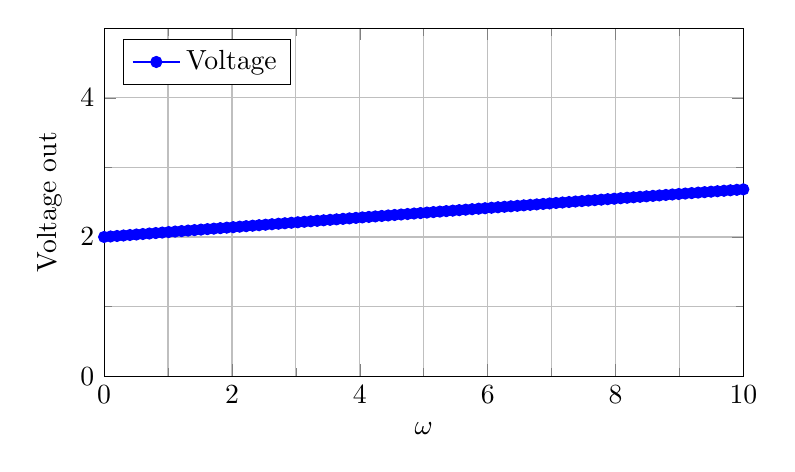
\begin{tikzpicture}
        \begin{axis}[
            xlabel={$\omega$},
            ylabel={Voltage out},
            xmin=0, xmax=10, % Set your desired x-axis limits
            ymin=0, ymax=5,  % Set your desired y-axis limits
            legend pos=north west, % Adjust legend position if needed
            grid=both, % Enable grid
            minor tick num=1, % Number of minor ticks between major ticks
            width=0.8\linewidth, % Adjust the width of the plot
            height=6cm, % Adjust the height of the plot
            ]
            
            \addplot[blue, mark=*, samples=100, domain=0:10] {2*sin(2*x)+2}; % Example function, replace with your data
            
            % Add more \addplot commands for additional data series if needed
            
            \legend{Voltage}
          \end{axis}
    \end{tikzpicture}
\end{figure}

Say we have a system like fig. \ref{fig:avgpow}. 
\begin{figure}
    \center
    \caption{Power}
    \label{fig:avgpow}
    \begin{circuitikz}[american voltages, european resistors]
        \draw (0,0) to[V, l=$\tilde{V}_{th}$, invert] (0,2)
        to[R, l=$Z_{th}$] (4,2)
        to[R, l=$Z_{L}$] (4,0)
        to[short] (0,0)
        ;
    \end{circuitikz}
\end{figure}
We are interested in finding the
load that extracts the maximum power. 
Recall that 
\[P_{load} = \frac{1}{2}R_{load}|\tilde{I}_{load}|^2.\]
The current through the circuit is 
\begin{align*}
    \tilde{I} &= \frac{\tilde{V}_{th}}{Z_{th} + Z_L} \\
    &= \frac{\tilde{V}_{th}}{R_{th} + R_{load} + j(X_{th} + X_{load})} \\
    |\tilde{I}| &= \frac{|\tilde{V}_{th}|}{\sqrt{(R_{th} + R_{load})^2+(X_{th} + X_{load})^2}}
\end{align*}
Ergo, 
\begin{align*}
    P_{load} &= \frac{R_{load}|\tilde{V}_{th}|^2}{2((R_{th} + R_{load})^2+(X_{th} + X_{load})^2)} \\
\end{align*}
Which has a maximum when $X_{load} = -X_{th}$ and gives us a maximum possible 
value of 
\[P_{load,max} = \frac{|\tilde{V}_{th}|^2}{8R_{th}}\]

\section{Magnetically coupled circuits}

Say we have a current-carrying loop, as in fig. \ref{fig:loop}. 
\begin{figure}
    \center 
    \caption{Flux}
    \label{fig:loop}
    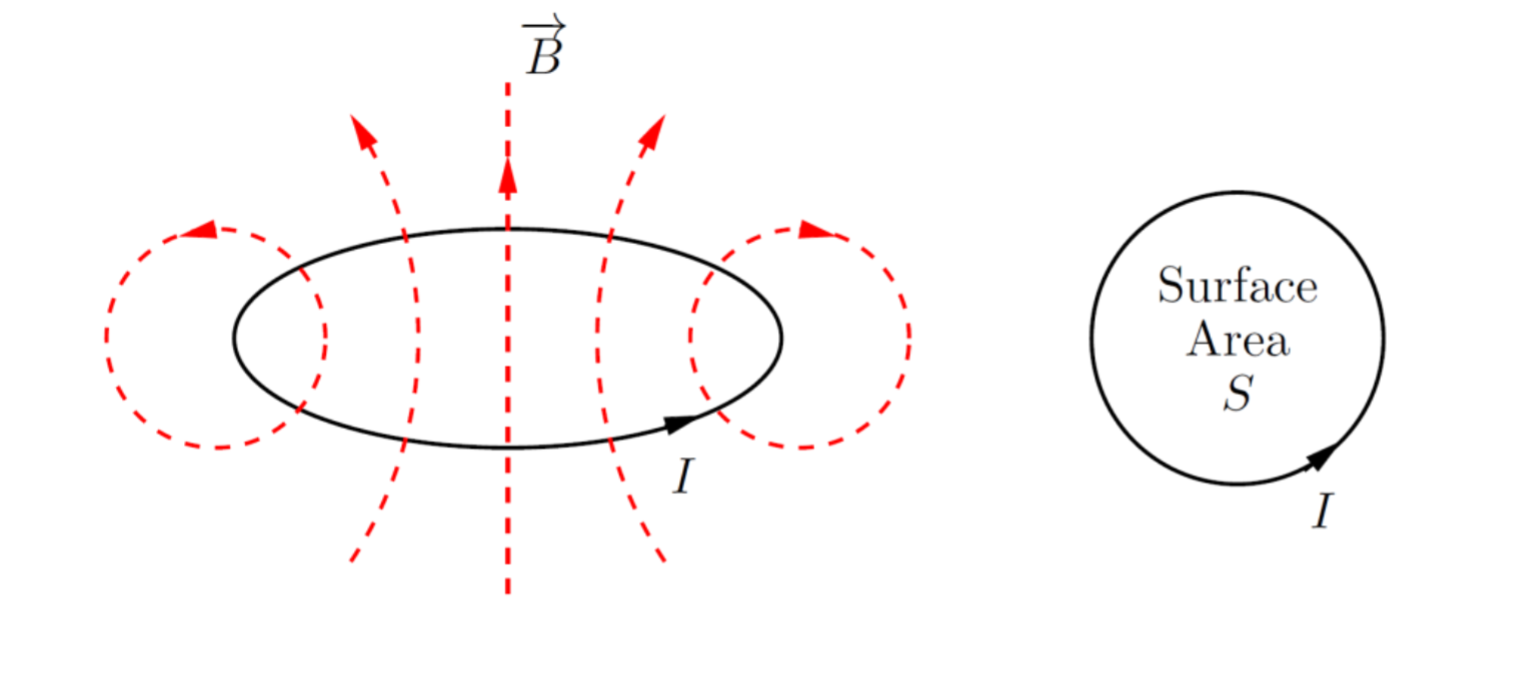
\includegraphics{images/Screenshot 2023-10-25 113639.png}
\end{figure}
The magnetic flux $\Phi$ is mathematically defined as 
\[\Phi = \int_{S} \vec{B} \cdot d\vec{S}.\]
Intuitively, flux is a measure of the total magnetic 
field which passes through a given area. 
We can also define the electromotive force (emf) as 
\[\epsilon = -\frac{d \Phi}{dt}\]
and the self-inductance as 
\[L = \frac{\Phi}{I}.\]
We can also have two loops near each other, as in fig. \ref{fig:mutual}.
\begin{figure}
    \center 
    \caption{Mutual inductance}
    \label{fig:mutual}
    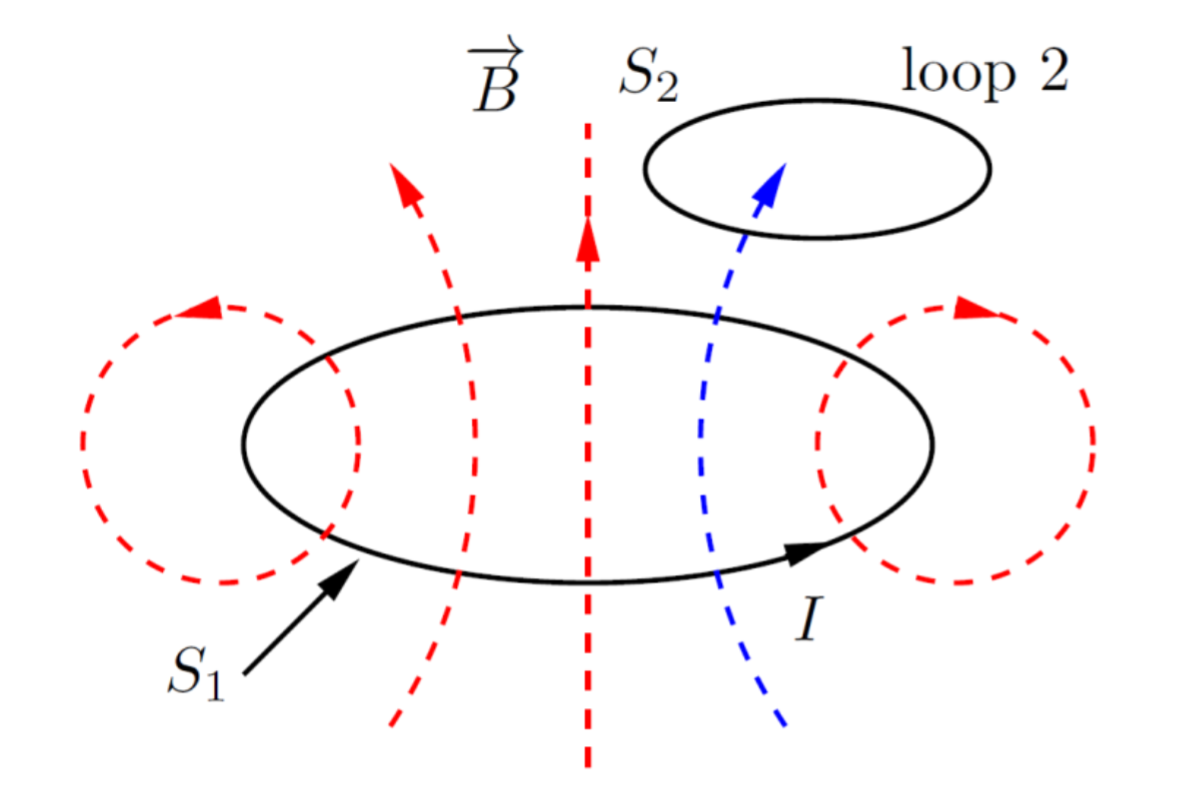
\includegraphics{images/mutualinductance.png}
\end{figure}
In this case, the flux through the second loop 
due to the current in the first is 
\[\Phi_{12} = \int_{S_2} \vec{B}_1 \cdot d\vec{S}_2.\]
Similarly as in the case where we had one loop, the 
\emph{mutual} inductance is defined as 
\[L_{12} = \frac{\Phi_{12}}{I_1}.\]
We can represent magnetically coupled coils as 
in fig. \ref{fig:coupled}. 
\begin{figure}
    \center 
    \caption{Coupled loops}
    \label{fig:coupled}
    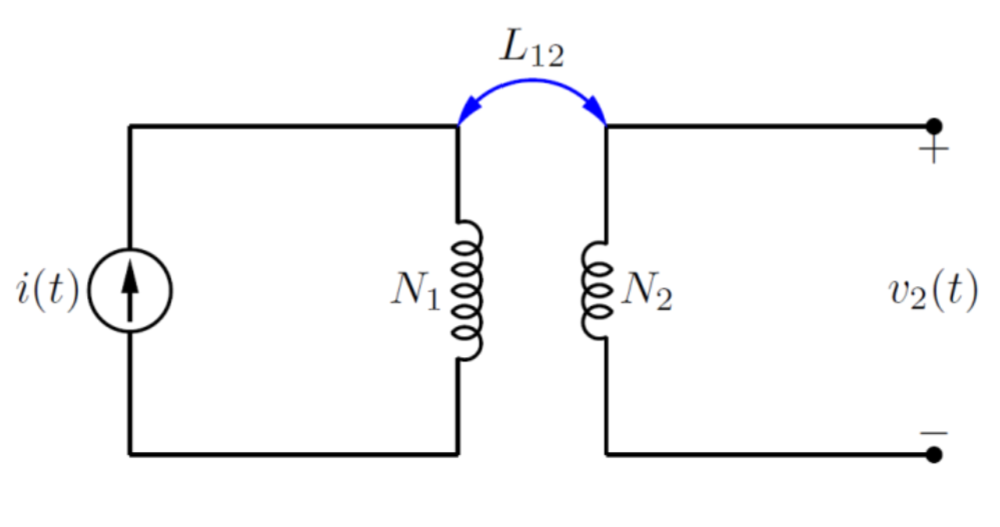
\includegraphics{images/coupledloops.png}
\end{figure}
and this system has a \emph{coupling coefficient} 
of $k = \frac{L_{12}}{\sqrt{L_1 L_2}}$.
Things can get messy when dealing with inductors, 
so to keep it straight, let's introduce the dot convention. 
The dot convention places a dot above an inductor and tells us 
that the current entering the dotted terminal of one
coil (inductor) induces a positive voltage oriented
towards the dotted terminal of the other coil.
We know that 
\begin{align*}
    v_{1}(t) &= L_1 \frac{di_1(t)}{dt} + L_{12}\frac{di_2(t)}{dt} \\
    v_{2}(t) &= L_1 \frac{di_2(t)}{dt} + L_{12}\frac{di_1(t)}{dt}
\end{align*}
and we can find the direction of the induced voltage using 
fig. \ref{fig:voltdir}
\begin{figure}
    \center 
    \caption{Voltage direction}
    \label{fig:voltdir}
    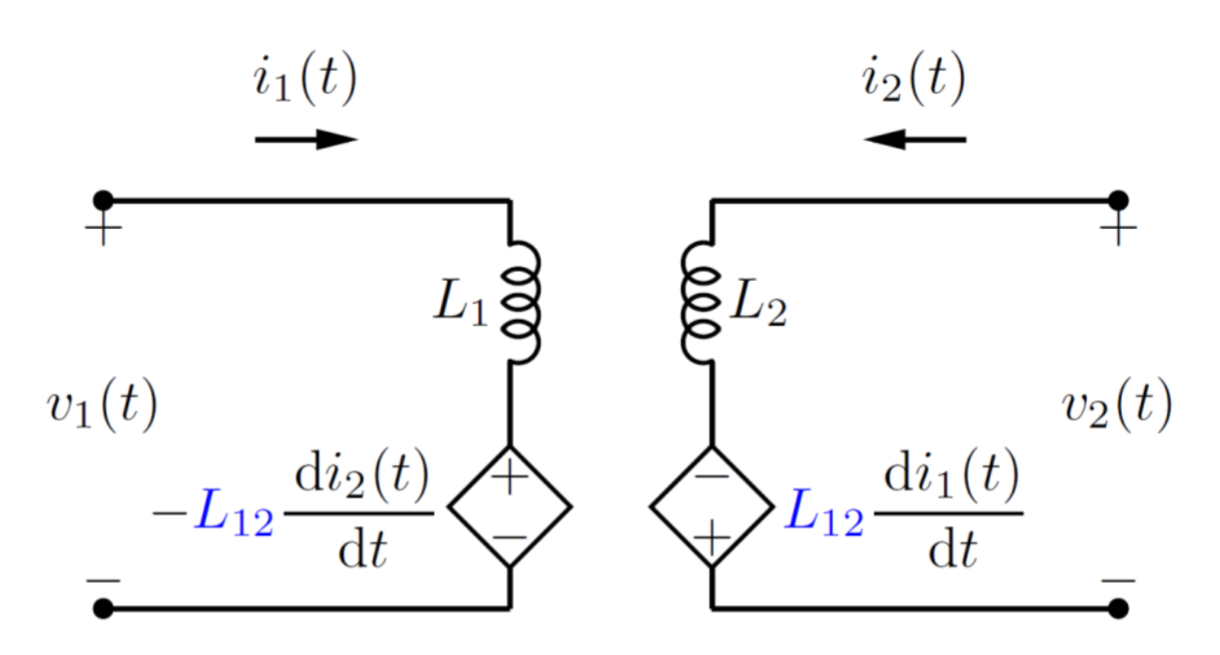
\includegraphics[width=\textwidth/2]{images/directionofinducedvoltage.png}
\end{figure}
The transformer is a component that uses magnetic coupling,
and is shown in fig. \ref{fig:transformer}. 
\begin{figure}
    \center 
    \caption{Transformer}
    \label{fig:transformer}
    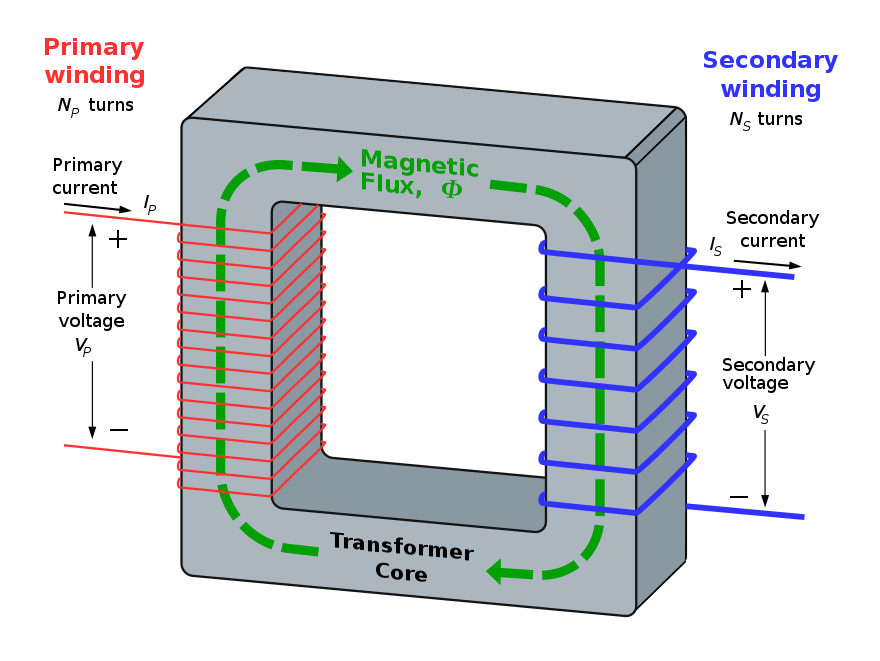
\includegraphics[width=\textwidth/2]{images/Transformer3d_col3.svg.png}
\end{figure}
The circuit diagram is shown in fig. \ref{fig:transschem}. 
\begin{figure}
    \center 
    \caption{Transformer schematic}
    \label{fig:transschem}
    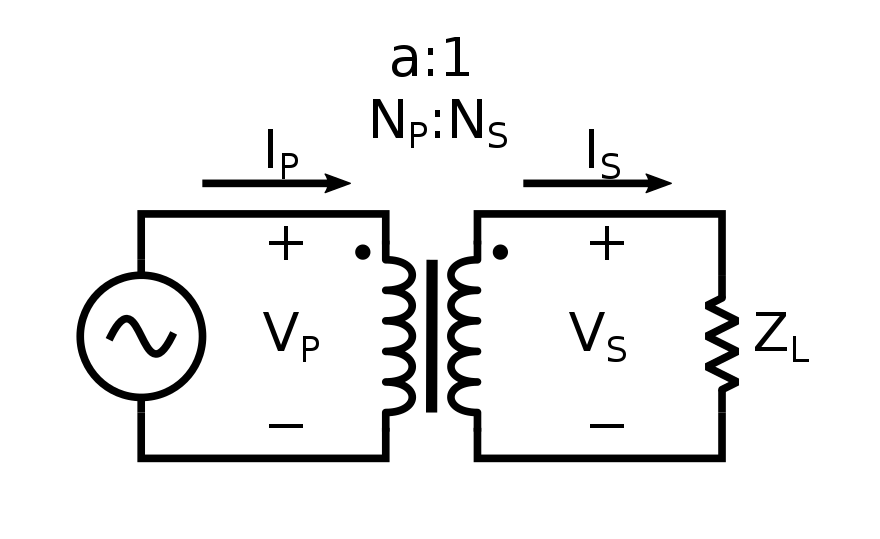
\includegraphics[width=\textwidth/2]{images/Ideal_transformer.svg.png}
\end{figure}
Interestingly, for transformers, the ratio of the voltages 
is equal to the ratio of the number of turns in each 
coil. That is, 
\[\frac{v_2(t)}{v_1(t)} = \frac{N_2}{N_1}.\]
We can also have a terminated transformer circuit, 
as shown in fig. \ref{fig:termtrans}. 
\begin{figure}
    \center 
    \caption{Terminated transformer}
    \label{fig:termtrans}
    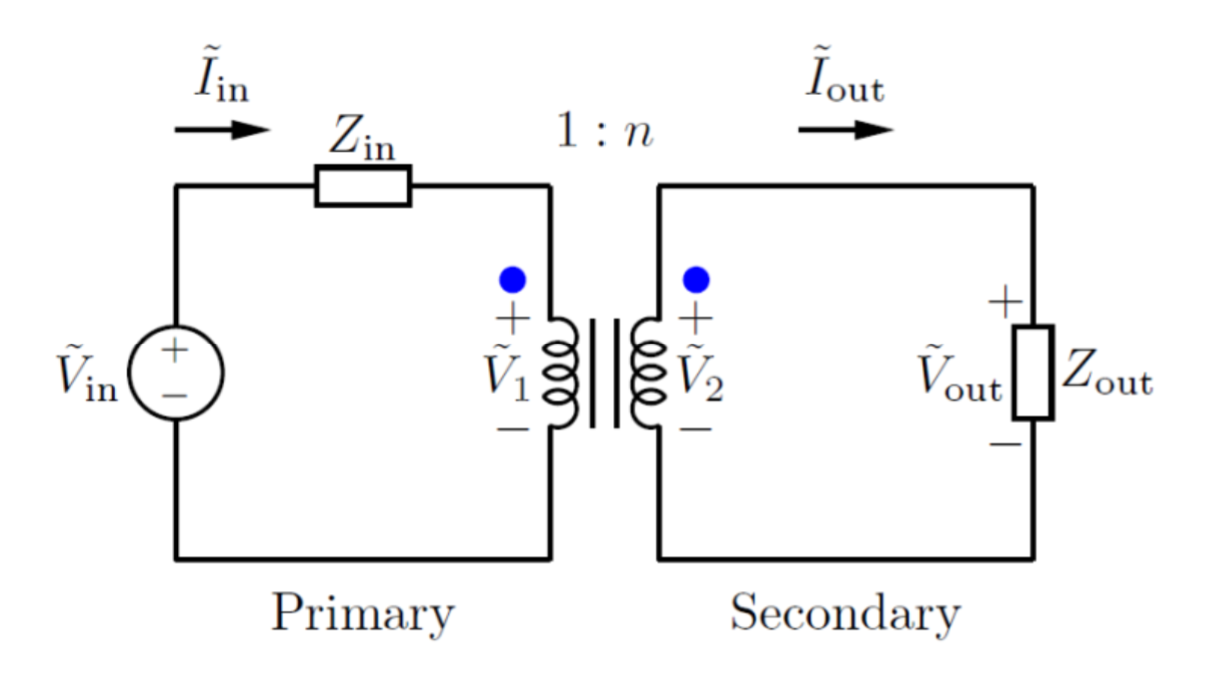
\includegraphics[width=\textwidth/2]{images/termtrans.png}
\end{figure}
In this case, we have that 
\begin{align*}
    \tilde{V}_{in} &= Z_{in} \tilde{I}_{in} + \tilde{V}_1 \\
    \tilde{V}_{2} &= Z_{out}\frac{\tilde{I}_{in}}{n} \\
    \frac{\tilde{V}_{in}}{\tilde{I}_{in}} &= Z_{in} + \frac{Z_{out}}{n^2}
\end{align*}
This final expression is the 
input impedance of a terminated 
ideal transformer. 

\section{Atomic structure and semiconductors}
All materials can be classified as insulators, semiconductors, 
or condcutors. We are familiar with insulators and conductors: 
the former does not conduct charge at all, while the latter 
is very good at conducting charge. Semiconductors lie in between 
in terms of conductivity. 

\defn{Semiconductors}{any of a class of crystalline 
solids intermediate in electrical conductivity 
between a conductor and an insulator}. 
Semiconductors can be elemental (silicon, germanium, etc.) or 
compounds (silicon carbide, gallium nitride, etc.). 

If we recall the structure of an atom, we will remember that 
there are discrete energy levels the electrons occupy. Adding energy to the system will 
move the electrons into a higher energy level. 
One of the most important materials in semiconducting is silicon, 
which luckily makes up around 28.2\% of the matter in the earth's crust. 
Silicon is a crystal with an atomic structure that makes it ideal 
for semiconducting. By adding energy to silicon, we can excite 
electrons in the orbitals of the atoms and cause them to flow along 
the material. When an electron flows away, it leaves behind a postively 
charged "hole". Electrons that are bound to atoms are in the "valence band",
while electrons free to flow are in the "conduction band". 
We can excite electrons by increasing the temperature 
of the material. If it is at 0 K, all electrons are 
in the valence band. If silicon is at room temperature, 
around $10^10$ electrons and locomoting about. 
For electrons to move between the valence
band and the conduction band, they need to cross the "band gap", 
which is the difference in energy between the top of the 
valence band and the bottom of the conduction band. Insulators have an 
extremely wide band gap, while conductors have an overlap 
between the conduction and valence bands. 
\begin{figure}
    \center
    \caption{Band gap for different types of materials}
    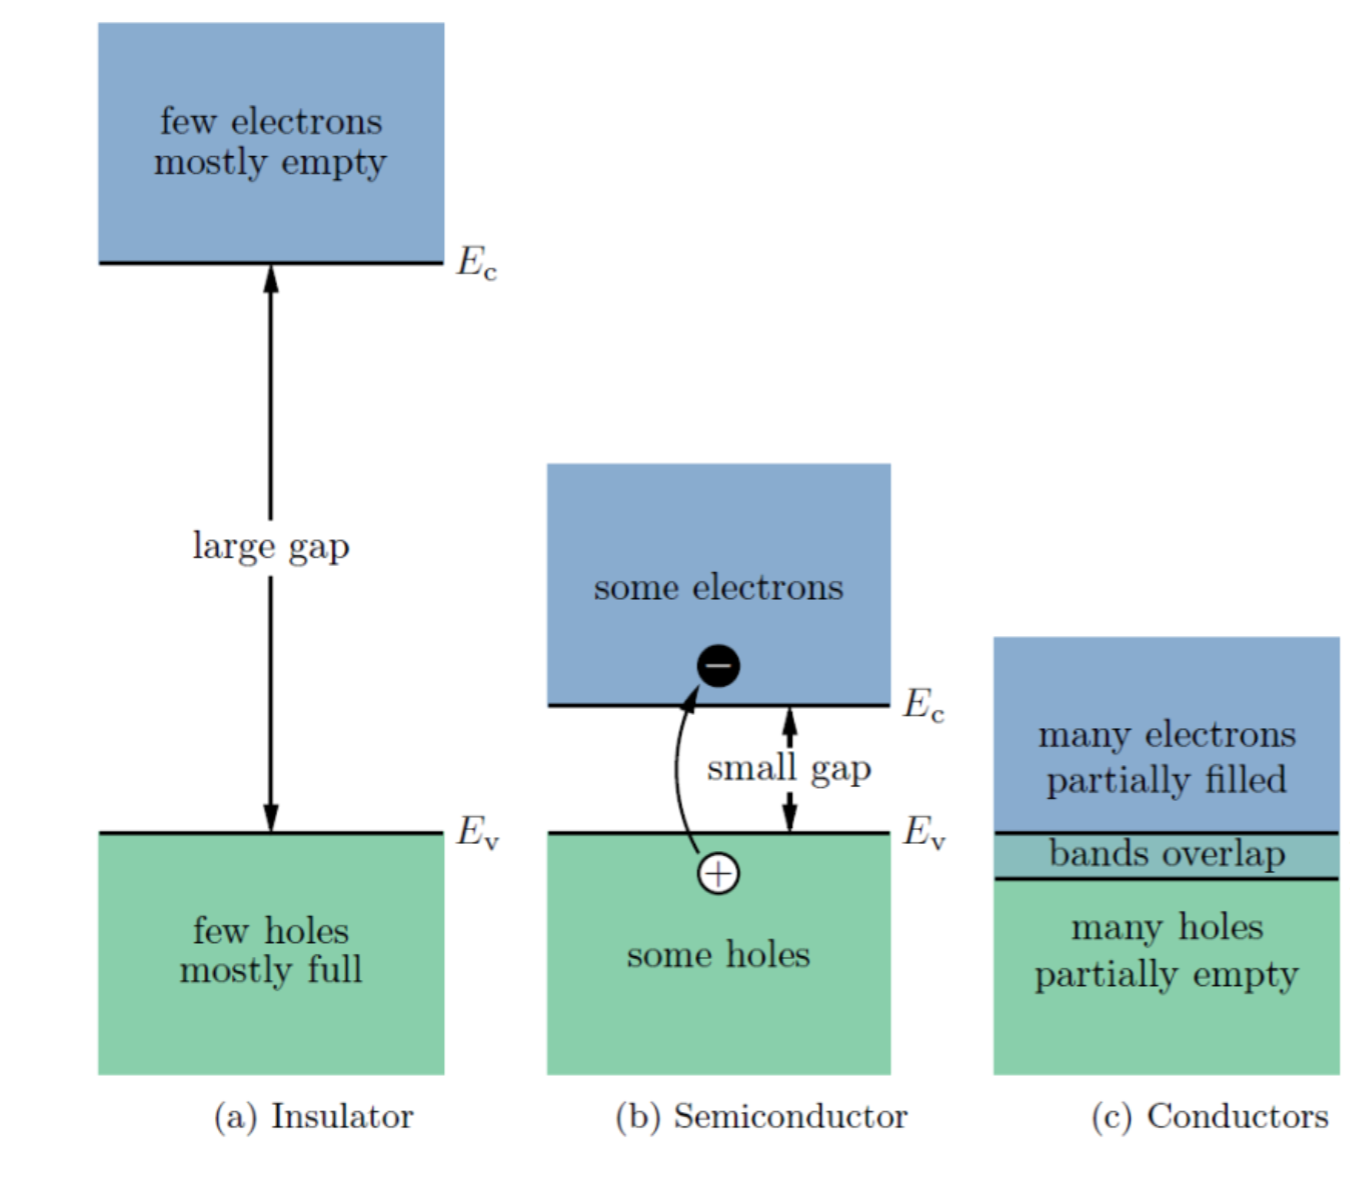
\includegraphics{images/bandgap}
\end{figure}
For silicon dioxide, the energy of the band gap is approximately 
$8 eV$. 

To summarize, 
\begin{itemize}
    \item The atomic structure of atoms influences the structure of their crystals. 
    \item The energy bands of materials determine their electrical properties. 
    \item In semiconductors, the valence and conduction band is seperated by the band gap. 
    \item Carrier density in intrinsic semiconductors increases with temperature. 
\end{itemize}

Intrinsic semiconductors are contrasted with \emph{doped} semiconductors. 

\defn{Doping}{intentionally
introducing useful impurities
into pure semiconductors}. 

\defn{Dopant}{intentionally introduced 
impurity}.

\defn{Donor}{dopant that donates free electron}. 

\defn{Acceptor}{dopant that accepts free electron}. 

Doped semiconductors, such as silicon doped with 
phosphorus, have improved electric conductivity. 
Since elemental phosphorus has one more electron than 
silicon, phosphorus donates an electron. 
\marginnote{It is no coincidence that the binding energy (the 
energy needed to seperate an electron) of phosphorus is much 
less than that of silicon.}
The positive charges caused by donors releasing an electron 
are not free to move about as the electron holes in silicon are. 
The cations are locked in the crystal lattice. 
At room temperature, almost all free electrons in a semiconductor 
are contributed by the dopant. Therefore, the number of 
free electrons in the crystal is approximately equal to 
the doping concentration. 
\[n \approx N_D\]

P-doping creates regions within the semiconductor with an excess of 
"holes" (missing electrons), which are the majority charge 
carriers in p-type (positive-type) semiconductors.

N-doping creates regions 
within the semiconductor with an excess of free 
electrons, which are the majority charge carriers 
in n-type (negative-type) semiconductors.

\defn{Recombination}{an electron (in
conduction band) and a hole (in valence
band) collide. The electron fills the hole,
giving off energy as a photon or phonon}.

\defn{Generation}{an electron (in the
valence band) absorbs energy and is
excited to the conduction band, leaving
behind a hole in the valence band}.

The recombination rate is proportional to the probability of an electron
(in the conduction band) colliding with a hole (in the valence band), 
which in turn is proportional to the number of holes and the number 
of free electrons. 
That is, 
\[\text{Recombination rate} \propto pn.\]
In equilibrium, the recombination rate equals the 
generation rate.
\[pn = n_i^2\]

\end{document}
